\setcounter{section}{1}
% Official AHL_2025__8__329_0.tex lines 312--330
\section{Definitions, notations and preliminaries}\label{s:preliminaries}



In the sequel, the letter $S$ will refer to a closed surface while the letter $\Sigma$ will refer to any surface (not necessarily compact, not necessarily connected). If $f$ is a surface homeomorphism, $\mu$ will refer to any $f$-invariant measure, $\lambda$ to an $f$-invariant measure with total support, and $\nu$ to an $f$-invariant ergodic measure.



\subsection{Loops and paths}\label{ss:loopsandpaths}



Let $\Sigma$ be an oriented surface (not necessarily closed, not necessarily boundaryless, not necessarily connected). A \emph{loop} of $\Sigma$ is a continuous map $\Gamma: \T\to \Sigma$, where $\T=\R/\Z$. It will be called \emph{essential} if it is not homotopic to a constant loop. A \emph{path} of $\Sigma$ is a continuous map $\gamma: I\to \Sigma$ where $I\subset \R$ is an interval. A loop or a path will be called \emph{simple} if it is injective. The \emph{natural lift} of a loop $\Gamma: \T\to \Sigma$ is the path $\gamma:\R\to \Sigma$ such that $\gamma(t)=\Gamma(t+\Z)$. A \emph{segment} is a simple path $\sigma:[a,b]\to \Sigma$, where $a<b$. The points $\sigma(a)$ and $\sigma(b)$ are the \emph{endpoints} of $\sigma$. We will say that $\sigma$ \emph{joins} $\sigma(a)$ to $\sigma(b)$. More generally if $A$ and $B$ are disjoint, we will say that $\sigma$ joins $A$ to $B$, if $\sigma(a)\in A$ and $\sigma(b)\in B$. A \emph{line} is a proper simple path $\lambda:\R\to \Sigma$. As it is usually done we will use the same name and the same notation to refer to the image of a loop or a path $\gamma$.

Note that a simple loop or a simple path is naturally oriented by its parametrization (the increasing one). Let $\Gamma$ be a simple loop of $\Sigma$, and denote $\Sigma'$ the connected component of $\Sigma$ it belongs to. If $\Sigma'\setminus\Gamma$ has two connected components, we say that $\Gamma$ \emph{separates} $\Sigma$; in this case the connected component that is located on the right of $\Gamma$ will be denoted $R(\Gamma)$ and the other one $L(\Gamma)$. We will use the same notations $R(\lambda)$, $L(\lambda)$ for a line $\lambda$ that separates the connected component it belongs to. In both cases, if $\gamma$ is a segment that joins $R(\Gamma)$ to $L(\Gamma)$, then it holds that the algebraic intersection number between $\Gamma$ and $\gamma$ is $1$.


Let $f$ be an orientation preserving homeomorphism of $\Sigma$. A \emph{Brouwer line} of $f$ is a line $\lambda$ that separates $\Sigma$ such that $f(\lambda)\subset L(\lambda)$ and $f^{-1}(\lambda)\subset R(\lambda)$. Equivalently it means that $f(\overline {L(\lambda)})\subset L(\lambda)$ or that $f^{-1}(\overline {R(\lambda)})\subset R(\lambda)$.


% Official AHL_2025__8__329_0.tex lines 399--578
\section{Foliations on surfaces}\label{s.foliations}



In this section we will consider an oriented boundaryless surface $\Sigma$, not necessarily closed, not necessarily connected, and a non singular oriented topological foliation $\F$ on $\Sigma$. We will consider:
\begin{itemize}
\item the universal covering space $\tilde\Sigma$ of $\Sigma$;
\item the covering projection $\tilde\pi: \tilde\Sigma\to \Sigma$;
\item the group ${\G}$ of covering automorphisms of this cover;
\item the lifted foliation $\tilde{\F}$ on $\tilde{\Sigma}$.
\end{itemize}

For every point $z\in\Sigma$, we denote $\phi_{z}$ the leaf of $\F$ that contains $z$. If $\phi_z:\R\to\Sigma$ is a parametrization of $\phi_z$ inducing the orientation, such that $\phi_z(0)=z$, we set $\phi_z^+=\phi_z\vert_{[0,+\infty)}$ and $\phi_z^-=\phi_z\vert_{(-\infty,0]}$. Similarly, for every point $\tilde z\in\tilde\Sigma$, we denote $\tilde\phi_{\tilde z}$ the leaf of $\tilde{\F}$ that contains $\tilde z$ and we define in the same way $\tilde\phi_{\tilde z}^+$ and $\tilde\phi_{\tilde z}^-$. The foliation $\tilde{\F}$ being defined on a union of topological planes and being non singular, it has no closed leaf. Moreover a leaf cannot accumulate on a point, it must be proper. So it is a line and consequently it separates the connected component of $\tilde{\Sigma}$ it belongs to (by Jordan theorem, because this connected component has to be a topological plane).



\subsection{\texorpdfstring{$\F$}{F}-transverse intersections}\label{ss.intersections}


A path $\gamma:J\to\Sigma$ is \emph {positively transverse}\footnote{In the whole text, ``transverse'' will mean ``positively transverse''.} to $\F$ if it locally crosses each leaf of $\F$ from the right to the left. Observe that every lift $\tilde\gamma:J\to\tilde\Sigma$ of $\gamma$ is positively transverse to $\tilde{\F}$ and that for every $a<b$ in $J$:
\begin{itemize}
\item $\tilde\gamma|_{[a,b]}$ meets once every leaf $\tilde\phi$ such that $R(\tilde\phi_{\tilde \gamma(a)})\subset R(\tilde\phi)\subset R(\tilde\phi_{\tilde \gamma(b)})$;
\item $\tilde\gamma|_{[a,b]}$ does not meet any other leaf.
\end{itemize}
Two transverse paths $\tilde\gamma_1:J_1\to\tilde\Sigma$ and $\tilde\gamma_2:J_2\to\tilde\Sigma$ are said \emph{equivalent} if they meet the same leaves of $\tilde{\F}$. Two transverse paths $\gamma_1:J_1\to\Sigma$ and $\gamma_2:J_2\to\Sigma$ are \emph{equivalent} if there exists a lift $\tilde\gamma_1:J_1\to\tilde\Sigma$ of $\gamma$ and a lift $\tilde\gamma_2:J_2\to\tilde\Sigma$ of $\gamma_2$ that are equivalent.

Let $\tilde\gamma_1:J_1\to \tilde\Sigma$ and $\tilde\gamma_2:J_2\to \tilde \Sigma$ be two transverse paths such that there exist $t_1\in J_1$ and $t_2\in J_2$ satisfying $\tilde\gamma_1(t_1)=\tilde\gamma_2(t_2)$. We will say that $\tilde\gamma_1$ and $\tilde\gamma_2$ have a \emph{$\tilde{\F}$-transverse intersection} at $\tilde\gamma_1(t_1)=\tilde\gamma_2(t_2)$ if there exist $a_1, b_1\in J_1$ satisfying $a_1<t_1<b_1$ and $a_2, b_2\in J_2$ satisfying $a_2<t_2<b_2$ such that:
\begin{itemize}
\item $\tilde\phi_{\tilde\gamma_1(a_1)}\subset L(\tilde\phi_{\tilde\gamma_2(a_2)}),\enskip \tilde\phi_{\tilde\gamma_2(a_2)}\subset L(\tilde\phi_{\widetilde\gamma_1(a_1)})$;

\item $\tilde\phi_{\widetilde\gamma_1(b_1)}\subset R(\tilde\phi_{\tilde\gamma_2(b_2)}),\enskip \tilde\phi_{\tilde\gamma_2(b_2)}\subset R(\tilde\phi_{\widetilde\gamma_1(b_1)})$;

\item every path joining $\tilde\phi_{\tilde\gamma_1(a_1)}$ to $\tilde\phi_{\tilde\gamma_1(b_1)}$ and every path joining $\tilde\phi_{\tilde\gamma_2(a_2)}$ to $\tilde\phi_{\tilde\gamma_2(b_2)}$ must intersect.
\end{itemize}

\begin{figure}
\begin{center}


\tikzset{every picture/.style={line width=0.6pt}}

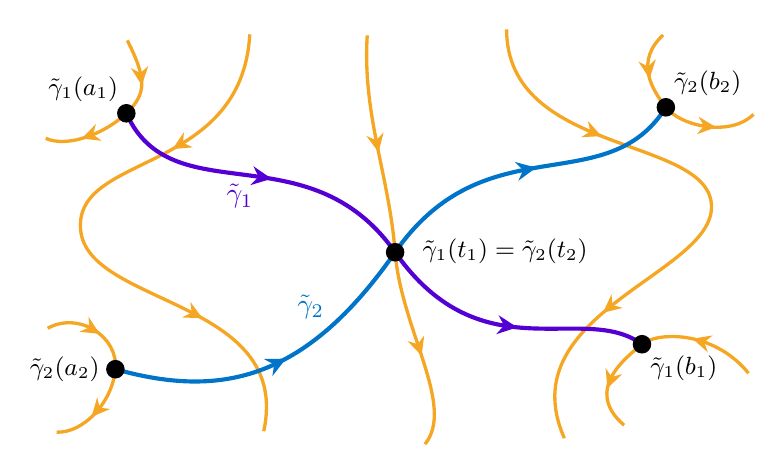
\begin{tikzpicture}[x=0.75pt,y=0.75pt,yscale=-1.1,xscale=1.1]

\draw [color={rgb, 255:red, 245; green, 166; blue, 35 },draw opacity=1] (261.43,50.73).. controls (259.25,85.76) and (271.02,112.03).. (273.64,145.74).. controls (276.25,179.45) and (300.23,213.16).. (286.72,229.8) ;
\draw [shift={(266.37,101.91)}, rotate = 258.81] [fill={rgb, 255:red, 245; green, 166; blue, 35 },fill opacity=1][line width=0.08] [draw opacity=0] (8.04,-3.86) -- (0,0) -- (8.04,3.86) -- (5.34,0) -- cycle ;
\draw [shift={(285.23,191.05)}, rotate = 251.75] [fill={rgb, 255:red, 245; green, 166; blue, 35 },fill opacity=1][line width=0.08] [draw opacity=0] (8.04,-3.86) -- (0,0) -- (8.04,3.86) -- (5.34,0) -- cycle ;
\draw [color={rgb, 255:red, 245; green, 166; blue, 35 },draw opacity=1] (156.35,52.92).. controls (164.64,69.56) and (165.07,76.12).. (155.92,84.88).. controls (146.76,93.64) and (130.19,100.2).. (120.6,95.83) ;
\draw [shift={(162.66,72.57)}, rotate = 263.3] [fill={rgb, 255:red, 245; green, 166; blue, 35 },fill opacity=1][line width=0.08] [draw opacity=0] (8.04,-3.86) -- (0,0) -- (8.04,3.86) -- (5.34,0) -- cycle ;
\draw [shift={(136.28,95.94)}, rotate = 340.46] [fill={rgb, 255:red, 245; green, 166; blue, 35 },fill opacity=1][line width=0.08] [draw opacity=0] (8.04,-3.86) -- (0,0) -- (8.04,3.86) -- (5.34,0) -- cycle ;
\draw [color={rgb, 255:red, 245; green, 166; blue, 35 },draw opacity=1] (391,50.6).. controls (378.79,61.98) and (385.69,73.93).. (392.23,82.25).. controls (398.77,90.57) and (420.57,95.39).. (430.6,85.32) ;
\draw [shift={(385.1,69.68)}, rotate = 262.21] [fill={rgb, 255:red, 245; green, 166; blue, 35 },fill opacity=1][line width=0.08] [draw opacity=0] (8.04,-3.86) -- (0,0) -- (8.04,3.86) -- (5.34,0) -- cycle ;
\draw [shift={(414.19,90.98)}, rotate = 185.63] [fill={rgb, 255:red, 245; green, 166; blue, 35 },fill opacity=1][line width=0.08] [draw opacity=0] (8.04,-3.86) -- (0,0) -- (8.04,3.86) -- (5.34,0) -- cycle ;
\draw [color={rgb, 255:red, 245; green, 166; blue, 35 },draw opacity=1] (209.98,50.29).. controls (206.49,112.03) and (133.24,101.96).. (135.86,135.67).. controls (138.48,169.38) and (228.73,165.88).. (216.09,224.11) ;
\draw [shift={(176.16,100.54)}, rotate = 329.51] [fill={rgb, 255:red, 245; green, 166; blue, 35 },fill opacity=1][line width=0.08] [draw opacity=0] (8.04,-3.86) -- (0,0) -- (8.04,3.86) -- (5.34,0) -- cycle ;
\draw [shift={(189.24,174.67)}, rotate = 208.12] [fill={rgb, 255:red, 245; green, 166; blue, 35 },fill opacity=1][line width=0.08] [draw opacity=0] (8.04,-3.86) -- (0,0) -- (8.04,3.86) -- (5.34,0) -- cycle ;
\draw [color={rgb, 255:red, 245; green, 166; blue, 35 },draw opacity=1] (322.47,48.1).. controls (322.47,103.27) and (410.46,94.79).. (412.2,125).. controls (413.94,155.21) and (323.34,172.01).. (347.76,227.17) ;
\draw [shift={(364.02,94.87)}, rotate = 202.65] [fill={rgb, 255:red, 245; green, 166; blue, 35 },fill opacity=1][line width=0.08] [draw opacity=0] (8.04,-3.86) -- (0,0) -- (8.04,3.86) -- (5.34,0) -- cycle ;
\draw [shift={(364.67,172.23)}, rotate = 320.57] [fill={rgb, 255:red, 245; green, 166; blue, 35 },fill opacity=1][line width=0.08] [draw opacity=0] (8.04,-3.86) -- (0,0) -- (8.04,3.86) -- (5.34,0) -- cycle ;
\draw [color={rgb, 255:red, 84; green, 0; blue, 213 },draw opacity=1][line width=1.5] (155.92,84.88).. controls (175.97,129.54) and (235.71,91.89).. (273.64,145.74).. controls (311.57,199.59) and (356.04,167.19).. (381.77,186.02) ;
\draw [shift={(219.54,113.55)}, rotate = 188.99] [fill={rgb, 255:red, 84; green, 0; blue, 213 },fill opacity=1][line width=0.08] [draw opacity=0] (8.75,-4.2) -- (0,0) -- (8.75,4.2) -- (5.81,0) -- cycle ;
\draw [shift={(327.1,178.63)}, rotate = 187.51] [fill={rgb, 255:red, 84; green, 0; blue, 213 },fill opacity=1][line width=0.08] [draw opacity=0] (8.75,-4.2) -- (0,0) -- (8.75,4.2) -- (5.81,0) -- cycle ;
\draw [color={rgb, 255:red, 0; green, 116; blue, 201 },draw opacity=1][line width=1.5] (151.12,196.96).. controls (196.46,209.66) and (233.96,202.65).. (273.64,145.74).. controls (313.31,88.82) and (366.07,123.85).. (392.23,82.25) ;
\draw [shift={(225.84,192.34)}, rotate = 153.5] [fill={rgb, 255:red, 0; green, 116; blue, 201 },fill opacity=1][line width=0.08] [draw opacity=0] (8.75,-4.2) -- (0,0) -- (8.75,4.2) -- (5.81,0) -- cycle ;
\draw [shift={(335.43,108.69)}, rotate = 169.41] [fill={rgb, 255:red, 0; green, 116; blue, 201 },fill opacity=1][line width=0.08] [draw opacity=0] (8.75,-4.2) -- (0,0) -- (8.75,4.2) -- (5.81,0) -- cycle ;
\draw [color={rgb, 255:red, 245; green, 166; blue, 35 },draw opacity=1] (121.47,179.01).. controls (134.99,171.57) and (152.43,182.51).. (151.12,196.96).. controls (149.81,211.41) and (137.17,224.98).. (125.4,224.55) ;
\draw [shift={(144.21,181.45)}, rotate = 211.25] [fill={rgb, 255:red, 245; green, 166; blue, 35 },fill opacity=1][line width=0.08] [draw opacity=0] (8.04,-3.86) -- (0,0) -- (8.04,3.86) -- (5.34,0) -- cycle ;
\draw [shift={(140.71,217.82)}, rotate = 311.55] [fill={rgb, 255:red, 245; green, 166; blue, 35 },fill opacity=1][line width=0.08] [draw opacity=0] (8.04,-3.86) -- (0,0) -- (8.04,3.86) -- (5.34,0) -- cycle ;
\draw [color={rgb, 255:red, 245; green, 166; blue, 35 },draw opacity=1] (428.42,198.71).. controls (412.72,179.45) and (387.87,180.76).. (381.77,186.02).. controls (375.66,191.27) and (355.61,205.72).. (373.92,221.48) ;
\draw [shift={(403.94,183.63)}, rotate = 16.09] [fill={rgb, 255:red, 245; green, 166; blue, 35 },fill opacity=1][line width=0.08] [draw opacity=0] (8.04,-3.86) -- (0,0) -- (8.04,3.86) -- (5.34,0) -- cycle ;
\draw [shift={(366.62,205.34)}, rotate = 290.52] [fill={rgb, 255:red, 245; green, 166; blue, 35 },fill opacity=1][line width=0.08] [draw opacity=0] (8.04,-3.86) -- (0,0) -- (8.04,3.86) -- (5.34,0) -- cycle ;
\draw [fill={rgb, 255:red, 0; green, 0; blue, 0 },fill opacity=1] (270.32,145.74).. controls (270.32,143.9) and (271.81,142.41).. (273.64,142.41).. controls (275.47,142.41) and (276.95,143.9).. (276.95,145.74).. controls (276.95,147.58) and (275.47,149.07).. (273.64,149.07).. controls (271.81,149.07) and (270.32,147.58).. (270.32,145.74) -- cycle ;
\draw [fill={rgb, 255:red, 0; green, 0; blue, 0 },fill opacity=1] (388.92,82.25).. controls (388.92,80.41) and (390.4,78.92).. (392.23,78.92).. controls (394.06,78.92) and (395.55,80.41).. (395.55,82.25).. controls (395.55,84.09) and (394.06,85.58).. (392.23,85.58).. controls (390.4,85.58) and (388.92,84.09).. (388.92,82.25) -- cycle ;
\draw [fill={rgb, 255:red, 0; green, 0; blue, 0 },fill opacity=1] (378.45,186.02).. controls (378.45,184.18) and (379.94,182.69).. (381.77,182.69).. controls (383.6,182.69) and (385.08,184.18).. (385.08,186.02).. controls (385.08,187.86) and (383.6,189.35).. (381.77,189.35).. controls (379.94,189.35) and (378.45,187.86).. (378.45,186.02) -- cycle ;
\draw [fill={rgb, 255:red, 0; green, 0; blue, 0 },fill opacity=1] (147.8,196.96).. controls (147.8,195.12) and (149.29,193.63).. (151.12,193.63).. controls (152.95,193.63) and (154.44,195.12).. (154.44,196.96).. controls (154.44,198.8) and (152.95,200.29).. (151.12,200.29).. controls (149.29,200.29) and (147.8,198.8).. (147.8,196.96) -- cycle ;
\draw [fill={rgb, 255:red, 0; green, 0; blue, 0 },fill opacity=1] (152.6,84.88).. controls (152.6,83.04) and (154.09,81.55).. (155.92,81.55).. controls (157.75,81.55) and (159.23,83.04).. (159.23,84.88).. controls (159.23,86.72) and (157.75,88.21).. (155.92,88.21).. controls (154.09,88.21) and (152.6,86.72).. (152.6,84.88) -- cycle ;

\draw (284.07,145.38) node [anchor=west] [inner sep=0.75pt] [font=\small] {$\tilde{\gamma }_{1}(t_{1}) =\tilde{\gamma }_{2}(t_{2})$};
\draw (205.68,114.4) node [anchor=north] [inner sep=0.75pt] [color={rgb, 255:red, 84; green, 0; blue, 213 },opacity=1] {$\tilde{\gamma }_{1}$};
\draw (244.15,176.67) node [anchor=south east] [inner sep=0.75pt] [color={rgb, 255:red, 0; green, 116; blue, 201 },opacity=1] {$\tilde{\gamma }_{2}$};
\draw (394.23,78.85) node [anchor=south west] [inner sep=0.75pt] [font=\small] {$\tilde{\gamma }_{2}(b_{2})$};
\draw (383.77,189.42) node [anchor=north west][inner sep=0.75pt] [font=\small] {$\tilde{\gamma }_{1}(b_{1})$};
\draw (145.8,196.96) node [anchor=east] [inner sep=0.75pt] [font=\small] {$\tilde{\gamma }_{2}(a_{2})$};
\draw (153.92,81.48) node [anchor=south east] [inner sep=0.75pt] [font=\small] {$\tilde{\gamma }_{1}(a_{1})$};
\end{tikzpicture}

\caption{Example of $\tilde{\F}$-transverse intersection.\label{Fig:extransverse}
}
\end{center}
\end{figure}

It means that there is a ``crossing'' between the two paths naturally defined by $\tilde\gamma_1$ and $\tilde\gamma_2$ in the space of leaves of $\widetilde{\F}$, which is a one-dimensional topological manifold, usually non Hausdorff (see Figure~\ref{Fig:extransverse}).


Now, let $\gamma_1:J_1\to \Sigma$ and $\gamma_2:J_2\to \Sigma$ be two transverse paths such that there exist $t_1\in J_1$ and $t_2\in J_2$ satisfying $\gamma_1(t_1)=\gamma_2(t_2)$. Say that $\gamma_1$ and $\gamma_2$ have a \emph{${\F}$-transverse intersection} at $\gamma_1(t_1)=\gamma_2(t_2)$ if $\tilde\gamma_1$ and $\tilde\gamma_2$ have a \emph{${\tilde{\F}}$-transverse intersection} at $\tilde\gamma_1(t_1)=\tilde\gamma_2(t_2)$, where $\tilde\gamma_1:J_1\to \tilde \Sigma$ and $\tilde\gamma_2:J_2\to \tilde \Sigma$ are lifts of $\gamma_1$ and $\gamma_2$ such that $\tilde\gamma_1(t_1)=\tilde\gamma_2(t_2)$. If $\gamma_1=\gamma_2$ one speaks of a \emph{$\F$-transverse self-intersection}. This means that if $\widetilde \gamma_1$ is a lift of $\gamma_1$, there exists $T\in\G$ such that $\widetilde\gamma_1$ and $T\widetilde\gamma_1$ have a $\widetilde{\F}$-transverse intersection at $\widetilde\gamma_1(t_1)=T\widetilde\gamma_1(t_2)$.



\subsection{Recurrence, equivalence and accumulation} A transverse path (with respect to the foliation $\F$) $\gamma:\R\to \Sigma$ is \emph{positively recurrent} if, for every $a<b$, there exist $c<d$, with $b<c$, such that $\gamma|_{[a,b]}$ and $\gamma|_{[c,d]}$ are equivalent. Similarly $\gamma$ is \emph{negatively recurrent} if, for every $a<b$, there exist $c<d$, with $d<a$, such that $\gamma|_{[a,b]}$ and $\gamma|_{[c,d]}$ are equivalent. Finally $\gamma$ is \emph{recurrent} if it is both positively and negatively recurrent.


Two transverse paths $\gamma_1:\R\to \Sigma$ and $\gamma_2:\R\to \Sigma$ are \emph{equivalent at $+\infty$} if there exists $a_1$ and $a_2$ in $\R$ such that $\gamma_1{}|_{[a_1,+\infty)}$ and $\gamma_2{}|_{[a_2,+\infty)}$ are equivalent. Similarly $\gamma_1$ and $\gamma_2$ are \emph{equivalent at $-\infty$} if there exists $b_1$ and $b_2$ in $\R$ such that $\gamma_1{}|_{(-\infty,b_1]}$ and $\gamma_2{}|_{(-\infty,b_2]}$ are equivalent.


A transverse path $\gamma_1:\R\to \Sigma$ \emph{accumulates positively} on the transverse path $\gamma_2:\R\to \Sigma$ if there exist real numbers $a_1$ and $a_2<b_2$ such that $\gamma_1{}|_{[a_1,+\infty)}$ and $\gamma_2{}|_{[a_2,b_2)}$ are equivalent. Similarly, $\gamma_1$ \emph{accumulates negatively} on $\gamma_2$ if there exist real numbers $b_1$ and $a_2<b_2$ such that $\gamma_1{}|_{(-\infty,b_1]}$ and $\gamma_2{}|_{(a_2,b_2]}$ are equivalent. Finally $\gamma_1$ \emph{accumulates} on $\gamma_2$ if it accumulates positively or negatively on $\gamma_2$.


\subsection{Strips} \label{ss:strips}

We fix $T\in {\G}\setminus\{0\}$ and consider
\begin{itemize}
\item the annulus $\hat\Sigma=\tilde\Sigma/T$ (or, if $\tilde\Sigma$ is not connected, the connected component of $\tilde\Sigma/T$ that is an annulus);
\item the covering projections $\pi: \tilde\Sigma\to \hat\Sigma$ and $\hat\pi: \hat\Sigma\to \Sigma$;
\item the foliation $\hat{\F}$ on $\hat{\Sigma}$ induced by $\tilde{\F}$.
\end{itemize}
Suppose that $\hat\Gamma_*$ is a simple loop transverse to $\hat{\F}$. Then, $\hat\Gamma_*$ is essential and $\tilde\gamma_*=\pi^{-1}(\hat\Gamma_*)$ can be seen as an oriented line of $\tilde \Sigma$, invariant by $T$ and transverse to $\tilde{\F}$. The set
\[
\hat B=\left\{\hat z \in \hat\Sigma \,\middle| \,\hat \phi_{\hat z} \cap \hat\Gamma_*\not=\emptyset\right\}
\]
is an open annulus which is $\hat{\F}$-saturated, meaning that it is a union of leaves. Similarly
\[
\tilde B=\pi^{-1}(\hat B)=\left\{\tilde z \in \tilde\Sigma\,\,\middle| \,\enskip \tilde\phi_{\tilde z} \cap \tilde\gamma_*\not=\emptyset\right\}
\]
is an $\tilde{\F}$-saturated plane invariant by $T$. We will call such a set a \emph{$T$-strip} (or a \emph{strip} if we do not want to specify the covering transformation). In other words a $T$-strip is a $\tilde{\F}$-saturated plane invariant by $T$ defined as the union of the leaves that meet a transverse line invariant by $T$.

The frontier of $\tilde B$, denoted $\partial \tilde B$, is a union of leaves (possibly empty) and can be written $\partial\tilde B=\partial\tilde B^R\sqcup\partial\tilde B^L$, where
\[
\partial\tilde B^R=\partial\tilde B\cap R(\tilde\gamma_*)\,,\qquad \partial\tilde B^L=\partial\tilde B\cap L(\tilde\gamma_*).
\]
Let us state some facts that can be proven easily (see~\cite [Lemme~2.1.7]{Lel}). Note first that:
\begin{itemize}
\item if there is a leaf $\tilde \phi\subset \partial\tilde B$ that is invariant by $T$, then the set $ \partial\tilde B^R$ or $ \partial\tilde B^L$ that contains $\tilde\phi$ is reduced to this leaf;
\item if $\tilde\gamma:\R\to\tilde\Sigma$ is transverse to $\tilde{\F}$, then the set of real numbers $t$ such that $\gamma(t)\in\tilde B$ is an open interval (possibly empty).
\end{itemize}
Suppose now that $\tilde\gamma:\R\to\tilde\Sigma$ is transverse to $\tilde{\F}$ and that
\[
\big\{ t\in\R\,\vert\enskip \gamma(t)\in\tilde B\big\}=(a,b),
\]
where $-\infty\leq a<b\leq\infty$. Say that
\begin{itemize}
\item $\tilde\gamma$ \emph{draws $\tilde B$} if there exist $t<t'$ in $(a,b)$ such that $\tilde\phi_{\tilde\gamma(t')}=T\tilde\phi_{\tilde\gamma(t))}$.
\end{itemize}


If, moreover, we suppose that $-\infty<a<b<+\infty$, say that:
\begin{itemize}
\item $\tilde\gamma$ \emph{crosses $\tilde B$ from the right to the left }if $\tilde\gamma(a)\in \partial\tilde B^R$ and $\tilde\gamma(b)\in \partial\tilde B^L$;
\item $\tilde\gamma$ \emph{crosses $\tilde B$ from the left to the right} if $\tilde\gamma(a)\in \partial\tilde B^L$ and $\tilde\gamma(b)\in \partial\tilde B^R$;
\item $\tilde\gamma$ \emph{visits $\tilde B$ on the right} if $\tilde\gamma(a)\in \partial\tilde B^R$ and $\tilde\gamma(b)\in \partial\tilde B^R$;
\item $\tilde\gamma$ \emph{visits $\tilde B$ on the left} if $\tilde\gamma(a)\in \partial\tilde B^L$ and $\tilde\gamma(b)\in \partial\tilde B^L$.
\end{itemize}
We will say that $\tilde\gamma$ \emph{crosses} $\tilde B$ if it crosses it from the right to the left or from the left to the right. Similarly, we will say that $\tilde\gamma$ \emph{visits} $\tilde B$ if it visits it on the right or on the left. Note that $T(\tilde\gamma)$ satisfies the same properties as $\tilde\gamma$. Note also that if $\tilde\gamma$ visits $\tilde B$ on the right, then $\partial \tilde B^R$ is not reduced to a $T$-invariant leaf. Indeed, suppose that $\partial \tilde B^R$ is reduced to a $T$-invariant leaf $\tilde\phi$. With the notations above, we know that $\tilde\gamma\vert_{(a,b)}$ is included in $L(\tilde \phi)$ because it is disjoint from $\tilde \phi$ and $\gamma(a)\in \tilde\phi$. Similarly, $\tilde\gamma\vert_{(a,b)}$ is included in $R(\tilde \phi)$ because it is disjoint from $\tilde \phi$ and $\gamma(b)\in \tilde\phi$. We have found a contradiction. An analogous property holds if $\tilde\gamma$ visits $\tilde B$ on the left. Let us state a lemma whose proof is straightforward.

\begin{lemm}\label{Lem4Possib}
At least one of the following situations occurs (the two last assertions are not incompatible):
\begin{itemize}
\item $\tilde\gamma$ crosses $\tilde B$;
\item $\tilde\gamma$ visits $\tilde B$;
\item $\tilde\gamma$ is equivalent to $\tilde \gamma_*$ at $+\infty$ or at $-\infty$;
\item $\tilde\gamma$ accumulates on $\tilde\gamma_*$ positively or negatively.
\end{itemize}
\end{lemm}

Let us conclude this list of properties by the following ones (see~\cite[Section~2.1.2.c]{Lel}):


\begin{prop}\label{prop:transversestrips}
We have the following results:
\begin{itemize}
\item If $\tilde\gamma$ visits and draws $\tilde B$, then $\tilde\gamma$ and $T(\tilde\gamma)$ have an $\tilde{\F}$-transverse intersection and so $\gamma=\tilde\pi\circ\tilde\gamma$ has an $\F$-transverse self intersection.

\item If $\tilde\gamma_1$ crosses $\tilde B$ from the right to the left, if $\tilde\gamma_2$ crosses $\tilde B$ from the left to the right and at least one of the paths $\tilde\gamma_1$ or $\tilde\gamma_2$ draws $\tilde B$, then there exists $k\in \Z$ such that $\tilde\gamma_1$ and $T^k(\tilde\gamma_2)$ have an $\tilde{\F}$-transverse intersection, and so $\gamma_1=\tilde\pi\circ\tilde\gamma_1$ and $\gamma_2=\tilde\pi\circ\tilde\gamma_2$ have an $\F$-transverse intersection.
\end{itemize}
\end{prop}



\subsection{More about the accumulation property}


In this final paragraph, we will suppose moreover than $\Sigma$ is connected and that $\Sigma\not=\R^2/\Z^2$. The goal is to prove the following result that has its own interest and will be used in the sequel to prove Theorem~\ref{th:main}. This statement is stronger than some results of~\cite[Section~2.1.1]{Lel}. It describes how a path $\gamma_1$ can accumulate on a path $\gamma_2$, the conclusion is that the situation depicted in Figure~\ref{fig:nontransitivity3} is more or less the only one that can occur.

% Official AHL_2025__8__329_0.tex lines 580--588
\begin{prop}\label{prop: nontransitivity3}
Suppose that $\gamma_1:\R\to \Sigma$ is a positively recurrent transverse path that accumulates positively on a transverse path $\gamma_2:\R\to \Sigma$. Then, there exists a transverse simple loop $\Gamma_*\subset\Sigma$ with the following properties.
\begin{enumerate}
\item The set $B$ of leaves met by $\Gamma_*$ is an open annulus of $\Sigma$.
\item The path $\gamma_1$ stays in $B$ and is equivalent to the natural lift of $\Gamma_*$.
\item If $\tilde\gamma_1$, $\tilde\gamma_2$ are lifts of $\gamma_1$, $\gamma_2$ to the universal covering space $\tilde\Sigma$ such that $\tilde\gamma_1\vert_{[a_1,+\infty)}$ is equivalent to $\tilde\gamma_2\vert_{[a_2,b_2)}$ and if $\tilde B$ is the lift of $B$ that contains $\tilde\gamma_1$, then one of the inclusions $\tilde\phi_{\tilde\gamma_2(b_2)}\subset \partial \tilde B^R$, $\tilde\phi_{\tilde\gamma_2(b_2)}\subset \partial \tilde B^L$ holds. In the first case, we have $\tilde B\subset L(\tilde \phi)$ for every $\tilde \phi\subset \partial \tilde B^R$ and in the second case, we have $\tilde B\subset R(\tilde \phi)$ for every $\tilde \phi\subset \partial \tilde B^L$.
\end{enumerate}
\end{prop}


% Official AHL_2025__8__329_0.tex lines 590--632
\begin{figure}
\begin{center}

\tikzset{every picture/.style={line width=0.75pt}}

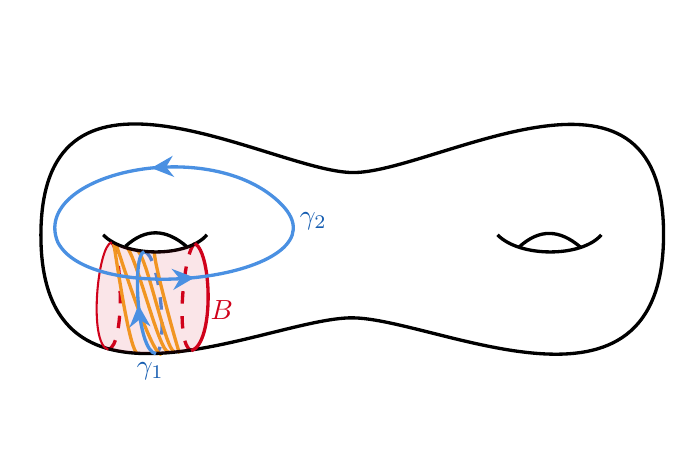
\begin{tikzpicture}[x=0.75pt,y=0.75pt,yscale=-1,xscale=1]
\draw [color={rgb, 255:red, 208; green, 2; blue, 27 },draw opacity=1] [dash pattern={on 4.5pt off 4.5pt}] (214.14,203.57).. controls (219,208.43) and (220.71,253.29).. (212.43,255.29) ;
\draw [color={rgb, 255:red, 208; green, 2; blue, 27 },draw opacity=1] [dash pattern={on 4.5pt off 4.5pt}] (254.14,204.14).. controls (248.71,207.86) and (244.43,252.71).. (252.43,255.86) ;
\draw [color={rgb, 255:red, 74; green, 144; blue, 226 },draw opacity=1] [dash pattern={on 4.5pt off 4.5pt}] (229.8,208.1).. controls (237.2,209.1) and (241.6,254.7).. (235.4,257.3) ;

\draw [color={rgb, 255:red, 245; green, 166; blue, 35 },draw opacity=1] (220.71,205.57).. controls (225.4,206.7) and (236.8,257.3).. (241.6,256.5) ;
\draw [color={rgb, 255:red, 245; green, 166; blue, 35 },draw opacity=1] (216.11,204.17).. controls (218.6,211.7) and (233.4,258.5).. (238.2,257.7) ;
\draw [color={rgb, 255:red, 245; green, 166; blue, 35 },draw opacity=1] (226.11,207.37).. controls (230.8,208.5) and (239.8,255.1).. (244.2,256.3) ;
\draw [color={rgb, 255:red, 245; green, 166; blue, 35 },draw opacity=1] (234.71,208.77).. controls (234.6,214.1) and (245.4,253.5).. (246.8,257.1) ;
\draw [color={rgb, 255:red, 245; green, 166; blue, 35 },draw opacity=1] (215,203.57).. controls (216.49,212.3) and (222.06,252.3).. (226.06,256.9) ;


\draw (180,200).. controls (180.2,101.4) and (291.4,169.4).. (330,170).. controls (368.6,170.6) and (480.2,101).. (480,200).. controls (479.8,299) and (369.8,240.2).. (330,240).. controls (290.2,239.8) and (179.8,298.6).. (180,200) -- cycle ;
\draw (210,200).. controls (220.6,211) and (250.6,211).. (260,200) ;
\draw (400,200).. controls (410.6,211) and (440.6,211).. (450,200) ;
\draw (220.71,205.57).. controls (230.57,196.57) and (240.29,197.14).. (250.14,205.57) ;
\draw (410.43,205.86).. controls (420.29,196.86) and (430,197.43).. (439.86,205.86) ;
\draw [color={rgb, 255:red, 208; green, 2; blue, 27 },draw opacity=1][line width=0.75] (214.14,203.57).. controls (207.29,205) and (202.71,252.71).. (212.43,255.29) ;
\draw [color={rgb, 255:red, 208; green, 2; blue, 27 },draw opacity=1] (254.14,204.14).. controls (262.43,208.71) and (263.57,252.43).. (252.43,255.86) ;

\fill [color={rgb, 255:red, 208; green, 2; blue, 27 },fill opacity=.1][line width=0.75] (214.14,203.57).. controls (207.29,205) and (202.71,252.71).. (212.43,255.29).. controls +(7,2) and +(-7,2).. (252.43,255.86).. controls +(263.57-252.43,252.43-255.86) and +(262.43-254.14,208.71-204.14).. (254.14,204.14).. controls +(-10,5) and +(10,5).. (214.14,203.57);

\draw [color={rgb, 255:red, 74; green, 144; blue, 226 },draw opacity=1] (188.14,203.57).. controls (205.29,236.71) and (329.57,219.57).. (295.86,185.29).. controls (262.14,151) and (174.43,170.43).. (188.14,203.57) -- cycle ;
\draw [shift={(254.01,220.61)}, rotate = 535.36] [fill={rgb, 255:red, 74; green, 144; blue, 226 },fill opacity=1][line width=0.08] [draw opacity=0] (10.72,-5.15) -- (0,0) -- (10.72,5.15) -- (7.12,0) -- cycle ;
\draw [shift={(233.23,167.82)}, rotate = 355.82] [fill={rgb, 255:red, 74; green, 144; blue, 226 },fill opacity=1][line width=0.08] [draw opacity=0] (10.72,-5.15) -- (0,0) -- (10.72,5.15) -- (7.12,0) -- cycle ;
\draw [color={rgb, 255:red, 74; green, 144; blue, 226 },draw opacity=1] (229.8,208.1).. controls (223.8,209.3) and (226.2,256.1).. (235.4,257.3) ;
\draw [shift={(227,233.78)}, rotate = 86.21] [fill={rgb, 255:red, 74; green, 144; blue, 226 },fill opacity=1][line width=0.08] [draw opacity=0] (10.72,-5.15) -- (0,0) -- (10.72,5.15) -- (7.12,0) -- cycle ;

\draw (303,187.65) node [anchor=north west][inner sep=0.75pt] [color={rgb, 255:red, 20; green, 92; blue, 176 },opacity=1] {$\gamma_2$};
\draw (224.5,259.65) node [anchor=north west][inner sep=0.75pt] [color={rgb, 255:red, 20; green, 92; blue, 176 },opacity=1] {$\gamma_1$};


\draw (260,230) node [anchor=north west][inner sep=0.75pt] [color={rgb, 255:red, 208; green, 2; blue, 27 },opacity=1] {$B$};
\end{tikzpicture}
\caption{An example where Proposition~\ref{prop: nontransitivity3} holds. \label{fig:nontransitivity3}
}
\end{center}
\end{figure}

% Official AHL_2025__8__329_0.tex lines 636--996
\begin{proof}
Note first that if $ \Gamma : \T\to\Sigma$ is a loop transverse to $\F$ and $\tilde\gamma : \R\to\widetilde \dom(I)$ is a lift of $\Gamma$, there exists $T\in \G$ such that $\tilde \gamma(t+1)=T(\tilde\gamma(t))$ for every $t\in\R$. The foliation $\F$ being non singular, there is no transverse loop. We deduce that $T$ is not the identity and that $\tilde\gamma$ is simple. The periodicity condition tells us that $\tilde \gamma$ is a line. So it defines naturally a $T$-strip, the union of leaves meeting $\tilde \gamma$. We will say that $T$ and $\tilde B$ are associated to $\tilde \gamma$.

Let us start with a lemma.

\pagebreak
\begin{lemm}\label{LemEquivSubpath}
Let $ \Gamma : \T\to\Sigma$ be a transverse loop and $\tilde\gamma : \R\to\widetilde \dom(I)$ a lift of~$\Gamma$. Let $T\in\G$ be the deck transformation associated to $\tilde \gamma$ and $\tilde B$ the $T$-strip associated to $\tilde\gamma$. Suppose that there exists a deck transformation $T'\in\G$ and $a\in\R$ such that $\tilde\gamma|_{[a,a+1]}$ is equivalent to a subpath of $T'\tilde\gamma$. Then $\tilde\gamma|_{[a,a+1)} \cap T'\tilde\gamma \neq \emptyset$. Moreover, if $\Gamma$ is a simple loop, then $T'\in\langle T\rangle$.
\end{lemm}


This lemma can be reduced easily to the following fact.

\begin{enonce}
{Sub-lemma}\label{SlemFoliationLoop}
Let $ \Gamma : \T\to\Sigma$ be a loop transverse to $\F$. Then, there exists $z\in\Gamma$ and $z'\in\Gamma$ such that $\phi_z^+$ does not meet $\Gamma$ but at the end point and $\phi_{z'}^-$ does not meet $\Gamma$ but at the end point.
\end{enonce}

\begin{proof}[Proof of Lemma~\ref{LemEquivSubpath}]
By Sublemma~\ref{SlemFoliationLoop}, there exist $z$, $z'$ in $\Gamma$ (possibly equal) such that $\phi_z^+$ and $\phi_{z'}^-$ do not meet $\Gamma$ but at their end point. Denote $\tilde z=\tilde\gamma(b)$, $\tilde z'=\tilde\gamma(b')$ the respective lifts of $z$, $z'$ that belong to $\tilde\gamma|_{[a,a+1)}$. There is no loss of generality by supposing that $b\leq b'$. The union of $\tilde\phi_{\tilde z}^+$, $\tilde\phi_{\tilde z'}^-$ and $\tilde\gamma([b,b'])$ defines a line of $\tilde\Sigma$ that separates $\tilde\phi_{\tilde z}^-\setminus\{\tilde z\}$ and $\tilde\phi_{\tilde z'}^+\setminus\{\tilde z'\}$. If $T'\tilde\gamma$ does not meet $\tilde\gamma([b,b'])$, then, by Sublemma~\ref{SlemFoliationLoop}, it does not meet this line. So (as by the hypothesis of the lemma it intersects both $\tilde\phi_{\tilde z}$ and $\tilde\phi_{\tilde z'}$) $T'\tilde\gamma$ must intersect $\tilde\phi_{\tilde z}^-\setminus\{\tilde z\}$ and $\tilde\phi_{\tilde z'}^+\setminus\{\tilde z'\}$, which contradicts the connectedness of $T'\tilde\gamma$ and the fact that it is disjoint from the line. We have got a contradiction. We conclude that $T'\tilde \gamma\cap \tilde\gamma|_{[a,a+1)}\neq \emptyset$.

In the case where $\Gamma$ is simple loop, we know that
\[
T'\tilde\gamma\cap\tilde\gamma\ne\emptyset\iff T'\tilde\gamma=\tilde\gamma \iff T'\in\langle T\rangle.\qedhere
\]
\end{proof}


\begin{proof}[Proof of Sublemma~\ref{SlemFoliationLoop}]
Fix $z\in\Gamma$. The loop $\Gamma$ being transverse to $\F$, there are finitely many parameters $t\in\T$ such that $z=\Gamma(t)$. Consequently, there exists a compact neighborhood $W_z$ of $z$, a homeomorphism $\Phi_z: W_z\to[-1,1]^2$ and a finite set $I_z$ such that:
\begin{itemize}
\item $\Phi_z$ sends $z$ onto $(0,0)$;
\item $\Phi_z$ sends $\F|_{ W_z}$ onto the vertical foliation oriented upward;
\item we have $\Phi_z(\Gamma\cap W_z)= \bigcup_{i\,\in\,I_z}\grr(\psi_{i,z})$, where $\psi_{i,z}: [-1,1]\to[-1,1]$ is a continuous function satisfying $\psi_{i,z}(0)=0$.
\end{itemize}
Here the notation $\grr(\psi)$ denotes the graph of $\psi:[-1,1]\to [-1,1]$ oriented from the right to the left. See Figure~\ref{FigLocalConfig} for an example of such a configuration.

\begin{figure}
\begin{center}

\tikzset{every picture/.style={line width=1.2pt}}

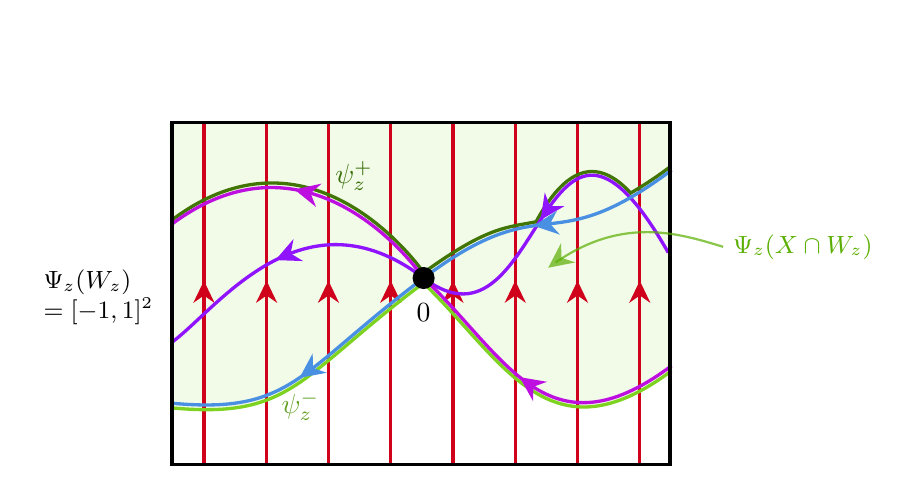
\begin{tikzpicture}[x=0.75pt,y=0.75pt,yscale=-1.5,xscale=1.5]

\draw [draw opacity=0][fill={rgb, 255:red, 126; green, 211; blue, 33 },fill opacity=0.1] (198.93,60.17).. controls (199,108.79) and (199.6,125.79).. (199.46,151.47).. controls (235,156.59) and (244.2,139.79).. (279.75,111.22).. controls (303.2,133.39) and (322,169.79).. (359.38,139.39).. controls (359.12,108.26) and (359.6,88.19).. (358.93,60.17) ;
\draw [color={rgb, 255:red, 208; green, 2; blue, 27 },draw opacity=1] (250,60) -- (250,170) ;
\draw [shift={(250,110.9)}, rotate = 90] [fill={rgb, 255:red, 208; green, 2; blue, 27 },fill opacity=1][line width=0.08] [draw opacity=0] (7.14,-3.43) -- (0,0) -- (7.14,3.43) -- (4.74,0) -- cycle ;
\draw [color={rgb, 255:red, 208; green, 2; blue, 27 },draw opacity=1] (270,60) -- (270,170) ;
\draw [shift={(270,110.9)}, rotate = 90] [fill={rgb, 255:red, 208; green, 2; blue, 27 },fill opacity=1][line width=0.08] [draw opacity=0] (7.14,-3.43) -- (0,0) -- (7.14,3.43) -- (4.74,0) -- cycle ;
\draw [color={rgb, 255:red, 208; green, 2; blue, 27 },draw opacity=1] (290,60) -- (290,170) ;
\draw [shift={(290,110.9)}, rotate = 90] [fill={rgb, 255:red, 208; green, 2; blue, 27 },fill opacity=1][line width=0.08] [draw opacity=0] (7.14,-3.43) -- (0,0) -- (7.14,3.43) -- (4.74,0) -- cycle ;
\draw [color={rgb, 255:red, 208; green, 2; blue, 27 },draw opacity=1] (310,60) -- (310,170) ;
\draw [shift={(310,110.9)}, rotate = 90] [fill={rgb, 255:red, 208; green, 2; blue, 27 },fill opacity=1][line width=0.08] [draw opacity=0] (7.14,-3.43) -- (0,0) -- (7.14,3.43) -- (4.74,0) -- cycle ;
\draw [color={rgb, 255:red, 208; green, 2; blue, 27 },draw opacity=1] (330,60) -- (330,170) ;
\draw [shift={(330,110.9)}, rotate = 90] [fill={rgb, 255:red, 208; green, 2; blue, 27 },fill opacity=1][line width=0.08] [draw opacity=0] (7.14,-3.43) -- (0,0) -- (7.14,3.43) -- (4.74,0) -- cycle ;
\draw [color={rgb, 255:red, 208; green, 2; blue, 27 },draw opacity=1] (350,60) -- (350,170) ;
\draw [shift={(350,110.9)}, rotate = 90] [fill={rgb, 255:red, 208; green, 2; blue, 27 },fill opacity=1][line width=0.08] [draw opacity=0] (7.14,-3.43) -- (0,0) -- (7.14,3.43) -- (4.74,0) -- cycle ;
\draw [color={rgb, 255:red, 208; green, 2; blue, 27 },draw opacity=1] (230.13,60) -- (230.13,170) ;
\draw [shift={(230.13,110.9)}, rotate = 90] [fill={rgb, 255:red, 208; green, 2; blue, 27 },fill opacity=1][line width=0.08] [draw opacity=0] (7.14,-3.43) -- (0,0) -- (7.14,3.43) -- (4.74,0) -- cycle ;
\draw [color={rgb, 255:red, 208; green, 2; blue, 27 },draw opacity=1] (210,60) -- (210,170) ;
\draw [shift={(210,110.9)}, rotate = 90] [fill={rgb, 255:red, 208; green, 2; blue, 27 },fill opacity=1][line width=0.08] [draw opacity=0] (7.14,-3.43) -- (0,0) -- (7.14,3.43) -- (4.74,0) -- cycle ;
\draw [color={rgb, 255:red, 126; green, 211; blue, 33 },draw opacity=1] (200.33,151.8).. controls (238.61,155.23) and (240.62,141.54).. (280.62,111.54) ;
\draw [color={rgb, 255:red, 126; green, 211; blue, 33 },draw opacity=1] (281.01,112.08).. controls (306.6,137.08) and (321.1,168.99).. (360.18,139.83) ;
\draw [color={rgb, 255:red, 65; green, 117; blue, 5 },draw opacity=1] (280.91,108.07).. controls (300.86,93.7) and (306.91,93.81).. (316.66,91.98).. controls (324.46,77.7) and (334.41,68.98).. (347.08,82.73).. controls (352.16,79.72) and (355.48,77.51).. (359.84,74.24) ;
\draw [color={rgb, 255:red, 144; green, 19; blue, 254 },draw opacity=1] (200.01,130.44).. controls (214.7,119.42) and (241.99,80.77).. (280.57,110.03).. controls (319.15,139.3) and (318.3,30.15).. (359.15,101.87) ;
\draw [shift={(232.96,104.27)}, rotate = 336.35] [fill={rgb, 255:red, 144; green, 19; blue, 254 },fill opacity=1][line width=0.08] [draw opacity=0] (8.04,-3.86) -- (0,0) -- (8.04,3.86) -- (5.34,0) -- cycle ;
\draw [shift={(318.13,91.36)}, rotate = 304.37] [fill={rgb, 255:red, 144; green, 19; blue, 254 },fill opacity=1][line width=0.08] [draw opacity=0] (8.04,-3.86) -- (0,0) -- (8.04,3.86) -- (5.34,0) -- cycle ;
\draw [color={rgb, 255:red, 65; green, 117; blue, 5 },draw opacity=1] (199.77,91.36).. controls (239.77,61.36) and (271.69,96.33).. (280.39,107.98) ;
\draw [color={rgb, 255:red, 74; green, 144; blue, 226 },draw opacity=1] (280.57,110.03).. controls (320.57,80.03) and (320.2,105.35).. (360.2,75.35) ;
\draw [shift={(315.89,93.26)}, rotate = 352.84] [fill={rgb, 255:red, 74; green, 144; blue, 226 },fill opacity=1][line width=0.08] [draw opacity=0] (8.04,-3.86) -- (0,0) -- (8.04,3.86) -- (5.34,0) -- cycle ;
\draw [color={rgb, 255:red, 74; green, 144; blue, 226 },draw opacity=1] (200.29,150.29).. controls (238.57,153.71) and (240.57,140.03).. (280.57,110.03) ;
\draw [shift={(240.71,142.08)}, rotate = 323.91] [fill={rgb, 255:red, 74; green, 144; blue, 226 },fill opacity=1][line width=0.08] [draw opacity=0] (8.04,-3.86) -- (0,0) -- (8.04,3.86) -- (5.34,0) -- cycle ;
\draw [color={rgb, 255:red, 189; green, 16; blue, 224 },draw opacity=1] (280.57,110.03).. controls (306.77,134.78) and (320.2,168.2).. (360.2,138.2) ;
\draw [shift={(311.43,141.87)}, rotate = 35.27] [fill={rgb, 255:red, 189; green, 16; blue, 224 },fill opacity=1][line width=0.08] [draw opacity=0] (8.04,-3.86) -- (0,0) -- (8.04,3.86) -- (5.34,0) -- cycle ;
\draw [color={rgb, 255:red, 189; green, 16; blue, 224 },draw opacity=1] (199.63,92.78).. controls (239.63,62.78) and (271.91,97.92).. (280.57,110.03) ;
\draw [shift={(239.09,81.59)}, rotate = 13.44] [fill={rgb, 255:red, 189; green, 16; blue, 224 },fill opacity=1][line width=0.08] [draw opacity=0] (8.04,-3.86) -- (0,0) -- (8.04,3.86) -- (5.34,0) -- cycle ;
\draw (199.71,60) -- (359.71,60) -- (359.71,170) -- (199.71,170) -- cycle ;
\draw [draw opacity=0][fill={rgb, 255:red, 0; green, 0; blue, 0 },fill opacity=1] (277.03,110.03).. controls (277.03,108.08) and (278.62,106.49).. (280.57,106.49).. controls (282.53,106.49) and (284.11,108.08).. (284.11,110.03).. controls (284.11,111.99) and (282.53,113.57).. (280.57,113.57).. controls (278.62,113.57) and (277.03,111.99).. (277.03,110.03) -- cycle ;
\draw [color={rgb, 255:red, 90; green, 174; blue, 0 },draw opacity=0.7][line width=0.8] (376.78,100).. controls (362.89,95.82) and (344.89,89.94).. (322.98,105.01) ;
\draw [shift={(320.58,106.73)}, rotate = 323.21] [fill={rgb, 255:red, 90; green, 174; blue, 0 },fill opacity=0.7][line width=0.08] [draw opacity=0] (8.04,-3.86) -- (0,0) -- (8.04,3.86) -- (5.34,0) -- cycle ;

\draw (280.57,116.97) node [anchor=north] [inner sep=0.75pt] {$0$};
\draw (241,145.33) node [anchor=north] [inner sep=0.75pt] [color={rgb, 255:red, 101; green, 160; blue, 37 },opacity=1] {$\psi _{z}^{-}$};
\draw (251,83) node [anchor=south west] [inner sep=0.75pt] [color={rgb, 255:red, 55; green, 110; blue, 5 },opacity=1] {$\psi _{z}^{+}$};
\draw (199.37,116.25) node [anchor=east] [inner sep=0.75pt] [font=\small] {$
\begin{array}{l}
\Psi _{z}(W_{z})\\
=[-1,1]^{2}
\end{array}$};
\draw (378.78,100) node [anchor=west] [inner sep=0.75pt] [font=\small,color={rgb, 255:red, 90; green, 174; blue, 0 },opacity=1] {$\Psi _{z}(X\cap W_{z})$};
\end{tikzpicture}
\caption{\label{FigLocalConfig}
Local configuration of the path $\Gamma$ and the foliation $\F$ (in red) around the point $0=\Psi_z(z)$ in Sublemma~\ref{SlemFoliationLoop}.}
\end{center}
\end{figure}

Consider the two continuous functions
\[
\psi_z^-=\min_{i\,\in\,I_z} \psi_{i,z}\,,\quad \psi_z^+=\max_{i\,\in\,I_z} \psi_{i,z}
\]
and define
\[
\gamma_z^{-}=\Phi_z^{-1}(\grr(\psi_z^-))\,,\quad\gamma_z^{+}=\Phi_z^{-1}(\grr(\psi_z^+)).
\]
We will argue by contradiction by supposing that for any $z\in\Gamma$, the path $\phi_z^+$ meets $\Gamma$ in a point that is not the end point. In that case, for every $z\in\Gamma$, there exists a sub-path $\delta_z:[0,1]\to\Sigma$ of $\phi_z^+$ such that
\[
\delta_z(0)=z,\quad
\delta_z(1)\in \Gamma,\quad
\delta_z((0,1))\cap\Gamma=\emptyset.
\]
In particular we can define a first return map $\theta:\Gamma\to\Gamma$ by setting $\theta(z)= \delta_z(1)$. We will prove that $X=\bigcup_{z\,\in\,\Gamma} \delta_z([0,1])$ is a compact sub-surface (possibly with boundary).


Note that for every $z\in\Gamma$, the function $\theta$ induces a homeomorphism from a neighborhood of $z$ in $\gamma_z^{+}$ to a neighborhood of $\theta(z)$ in $\gamma_{\theta(z)}^{-}$ and consequently that every point $\delta_z(t)$, $ t\in(0,1)$, belongs to the interior of $X$. Moreover, reducing the $W_z$ if necessary, one can suppose that $\theta$ is continuous on $\gamma_z^{+}$ and that $X_z=\bigcup_{z'\,\in\,\gamma_z^{+}} \delta_{z'}([0,1])$ is compact. The compact set
\[
X'_z=\Phi^{-1}_z\Big(\big\{(x,y)\in[0,1]^2\,\big|\, \psi_{z}^{-1}(x)\leq y\leq \psi_z^{+}(x)\big\}\Big)
\]
satisfies the equality
\[
X'_z\setminus\{z\}= \bigcup_{z'\,\in\,(W_z\,\cap\,\Gamma)\setminus \gamma_z^{+}} \delta_{z'}([0,1]),
\]
which implies that
\[
\bigcup_{z'\,\in\,W_z\,\cap\,\Gamma} \delta_{z'}([0,1])= X_z\cup X'_z.
\]
The loop $\Gamma$ can be covered by finitely many $W_z$, $z\in\Gamma$, and so $X$ is compact. By compactness of $X$, reducing the $W_z$ if necessary, one can suppose that the following alternative holds:
\begin{enumerate}
\item either $\gamma^-_z$ is contained in the image of $\theta$ and $W_z$ is included in $X$,

\item or $\gamma^-_z$ is disjoint from the image of $\theta$ and we have
\[
X\cap W_z=\Phi^{-1}_z\Big(\big\{(x,y)\in[0,1]^2\,\big|\, \psi_{z}^{-1}(x)\leq y\leq 1\big\}\Big).
\]
\end{enumerate}
The fact that every point $\delta_z(t)$, $z\in\Gamma$, $ t\in(0,1)$, belongs to the interior of $X$ implies that every point $z$ of the frontier of $X$ belongs to $\Gamma$. Moreover $W_z$ satisfies the second property. We have proved that $X$ is a compact sub-surface (possibly with boundary). Note that for every $z\in\partial X$ it holds that $\phi_z^+\setminus\{z\}\subset \intt(X)$ (in other terms the foliation is pointing inward on the boundary).

By hypothesis, $\Sigma$ is connected and different from $\R^2/\Z^2$. So, it does not bear a non-singular foliation. We deduce that $X$ is a surface with boundary. More precisely it is homeomorphic to the closed annulus because it bears a non singular foliation. Let $\Psi: X\to\S^2$ be a topological embedding compatible with the usual orientations. The loop $\Psi(\Gamma)$ is homologous to $0$ in $\S^2$ and one can define a dual function $\eta:\S^2\setminus\Psi(\Gamma)\to\Z$. Such a function is defined by the following property: for every $z$, $z'$ in $\S^2\setminus\Psi(\Gamma)$ and every path $\beta$ joining $z$ to $z'$, the algebraic intersection number $\Psi(\Gamma)\wedge \beta$ is equal to $\eta(z')-\eta(z)$. Let $U$ be a connected component of $\S^2\setminus\Psi(\Gamma)$ where $\eta$ reaches its maximum. The set $\Psi(\Gamma)$ being connected, the closure of $U$ is a topological disk. Moreover the fact that $\eta$ reaches its maximum in $U$ implies that for every $z\in \partial U$ it holds that $\phi_z^+\setminus\{z\}\subset U$. So $U$ is not a connected component of $\S^2\setminus \Psi(X)$ and it holds that $\overline U\subset \psi(X)$. Summarizing, we have found a closed topological disk bearing a non-singular foliation pointing inward on the boundary. We have got a contradiction.
\end{proof}



Let us explain how to construct the simple loop $\Gamma_*$, associated to $\gamma_1$, that appears in Proposition~\ref{prop: nontransitivity3}. As $\gamma_1$ is positively recurrent, there exist two numbers $c_1<c'_1$, with $c_1>a_1$, such that $\phi_{\gamma_1(c_1)} = \phi_{\gamma_1(c'_1)}$ (see Figure~\ref{Fignontransitivity3} for these different points). It implies that $\gamma_1\vert_{[c_1,c'_1]}$ is equivalent to a transverse path $\gamma_* :[c_1,c'_1]\to\Sigma $ such that $\gamma_*(c_1) = \gamma_*(c'_1)$. To get $\gamma_*$, one can modify $\gamma_1$ on a left neighborhood of $c'_1$, the modification taking place in a flow box containing the segment of leaf joining $\gamma_1(c_1)$ to $\gamma_1(c'_1)$. The set
\[
X=\big\{(t,t')\in [c_1,c'_1]^2\,\big\vert\, \enskip t<t'\enskip\text{and}\enskip \gamma_*(t) = \gamma_*(t')\big\}
\]
is non empty (because it contains $(c_1,c'_1)$) and compact. Indeed, it is closed in $\{(t,t')\in [c_1,c'_1]^2\,\vert \enskip t<t'\}$, an its closure in the compact set $\{(t,t')\in [c_1,c'_1]^2\,\vert \enskip t\leq t'\}$ does not contain any couple $(t,t)$. The function $(t,t')\mapsto t'-t$ being continuous and positive on $X$, reaches its minimum at a couple $(c''_1,c'''_1)$. So, replacing $(c_1,c'_1)$ with $(c''_1, c'''_1)$ if necessary, one can always suppose that $\gamma_*(t)\not=\gamma_*(t')$ if $t<t'$ and $(t,t')\not=(c_1,c'_1)$. One defines a continuous map $\Gamma_*:\T\to\S$ by setting $\Gamma_*(t+\Z)=\gamma_*((1-t)c_1+tc'_1)$ if $t\in[0,1]$. This map being injective, it is a simple loop transverse to $\F$. We denote $B$ the union of leaves met by $\Gamma_*$.

By hypothesis there exist two lifts $\tilde\gamma_1$ and $\tilde\gamma_2$ of respectively $\gamma_1$ and $\gamma_2$ to $\tilde\Sigma$ such that $\tilde\gamma_1|_{[a_1, +\infty)}$ and $\tilde\gamma_2|_{[a_2, b_2)}$ are equivalent. We denote $\tilde \gamma_*$ the lift of $\Gamma_*$ that contains $\tilde\gamma_1(c_1)$. Then we consider the deck transformation $T$ and the $T$-strip $\tilde B$ associated to $\tilde\gamma_*$. Note that $T$ is primitive because $\Gamma_*$ is simple.

\begin{lemm}\label{LemInclus}
The path $\tilde\gamma_1|_{[c_1,+\infty)}$ is included in $\tilde B$.
\end{lemm}

\begin{proof}
We will argue by contradiction and suppose it is not. Then there exists $d_1>c'_1$, uniquely defined, such that $\tilde\gamma_1(d_1)\notin\tilde B$ and $\tilde\gamma_1\vert_{[c_1,d_1)}\subset\tilde B$ (see Figure~\ref{Fignontransitivity3}).

\begin{figure}
\begin{center}
\tikzset{every picture/.style={line width=0.75pt}}

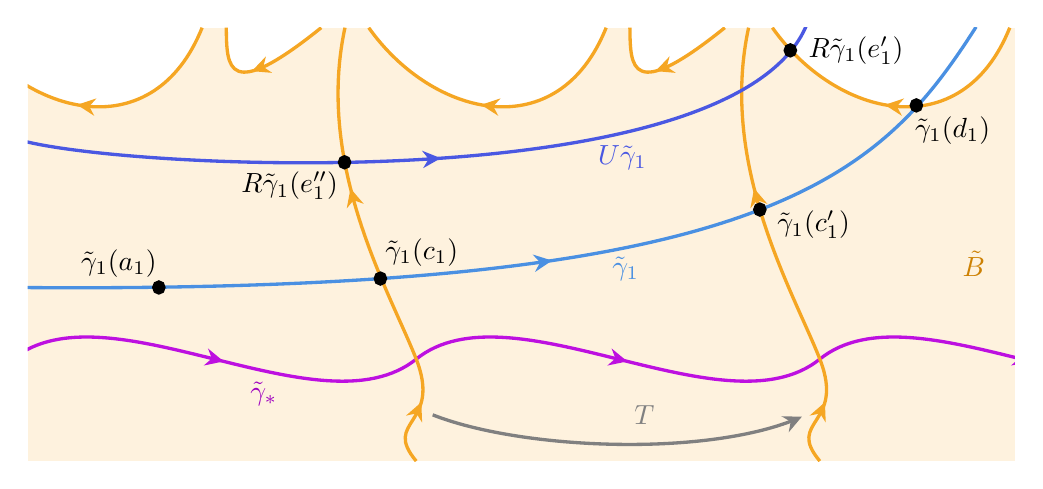
\begin{tikzpicture}[x=0.75pt,y=0.75pt,yscale=-1.1,xscale=1.1]
\clip (36.6,30.17) rectangle (469,220) ;

\draw [draw opacity=0][fill={rgb, 255:red, 245; green, 166; blue, 35 },fill opacity=0.15] (36.6,30.17) -- (469,30.17) -- (469,220) -- (36.6,220) -- cycle ;
\draw [color={rgb, 255:red, 245; green, 166; blue, 35 },draw opacity=1][fill={rgb, 255:red, 255; green, 255; blue, 255 },fill opacity=1] (185.98,30.17).. controls (214.06,69.7) and (268.96,82.65).. (289.97,30.17) ;
\draw [shift={(235.25,63.96)}, rotate = 7.23] [fill={rgb, 255:red, 245; green, 166; blue, 35 },fill opacity=1][line width=0.08] [draw opacity=0] (8.04,-3.86) -- (0,0) -- (8.04,3.86) -- (5.34,0) -- cycle ;
\draw [color={rgb, 255:red, 245; green, 166; blue, 35 },draw opacity=1][fill={rgb, 255:red, 255; green, 255; blue, 255 },fill opacity=1] (300.37,30.17).. controls (300.57,47.36) and (300.37,63.67).. (341.96,30.17) ;
\draw [shift={(311.58,49.2)}, rotate = 339.28] [fill={rgb, 255:red, 245; green, 166; blue, 35 },fill opacity=1][line width=0.08] [draw opacity=0] (8.04,-3.86) -- (0,0) -- (8.04,3.86) -- (5.34,0) -- cycle ;
\draw [color={rgb, 255:red, 245; green, 166; blue, 35 },draw opacity=1][fill={rgb, 255:red, 255; green, 255; blue, 255 },fill opacity=1] (362.76,30.17).. controls (390.83,69.7) and (445.74,82.65).. (466.75,30.17) ;
\draw [shift={(412.02,63.96)}, rotate = 7.23] [fill={rgb, 255:red, 245; green, 166; blue, 35 },fill opacity=1][line width=0.08] [draw opacity=0] (8.04,-3.86) -- (0,0) -- (8.04,3.86) -- (5.34,0) -- cycle ;
\draw [color={rgb, 255:red, 245; green, 166; blue, 35 },draw opacity=1][fill={rgb, 255:red, 255; green, 255; blue, 255 },fill opacity=1] (123.59,30.17).. controls (123.8,47.36) and (123.59,63.67).. (165.18,30.17) ;
\draw [shift={(134.8,49.2)}, rotate = 339.28] [fill={rgb, 255:red, 245; green, 166; blue, 35 },fill opacity=1][line width=0.08] [draw opacity=0] (8.04,-3.86) -- (0,0) -- (8.04,3.86) -- (5.34,0) -- cycle ;
\draw [color={rgb, 255:red, 189; green, 16; blue, 224 },draw opacity=1] (206.78,175.33).. controls (248.37,141.83) and (341.96,208.83).. (383.56,175.33) ;
\draw [shift={(299.22,176.34)}, rotate = 193.9] [fill={rgb, 255:red, 189; green, 16; blue, 224 },fill opacity=1][line width=0.08] [draw opacity=0] (8.04,-3.86) -- (0,0) -- (8.04,3.86) -- (5.34,0) -- cycle ;
\draw [color={rgb, 255:red, 189; green, 16; blue, 224 },draw opacity=1] (383.56,175.33).. controls (425.15,141.83) and (518.74,208.83).. (560.33,175.33) ;
\draw [shift={(476,176.34)}, rotate = 193.9] [fill={rgb, 255:red, 189; green, 16; blue, 224 },fill opacity=1][line width=0.08] [draw opacity=0] (8.04,-3.86) -- (0,0) -- (8.04,3.86) -- (5.34,0) -- cycle ;
\draw [color={rgb, 255:red, 189; green, 16; blue, 224 },draw opacity=1] (30,175.33).. controls (71.59,141.83) and (165.18,208.83).. (206.78,175.33) ;
\draw [shift={(122.44,176.34)}, rotate = 193.9] [fill={rgb, 255:red, 189; green, 16; blue, 224 },fill opacity=1][line width=0.08] [draw opacity=0] (8.04,-3.86) -- (0,0) -- (8.04,3.86) -- (5.34,0) -- cycle ;
\draw [color={rgb, 255:red, 245; green, 166; blue, 35 },draw opacity=1] (175.58,30.17).. controls (162.48,90.69) and (195.34,146.08).. (206.78,175.33).. controls (218.22,204.59) and (191.6,201.91).. (206.78,220) ;
\draw [shift={(178,100.57)}, rotate = 75.04] [fill={rgb, 255:red, 245; green, 166; blue, 35 },fill opacity=1][line width=0.08] [draw opacity=0] (8.04,-3.86) -- (0,0) -- (8.04,3.86) -- (5.34,0) -- cycle ;
\draw [shift={(209.01,194.24)}, rotate = 113.35] [fill={rgb, 255:red, 245; green, 166; blue, 35 },fill opacity=1][line width=0.08] [draw opacity=0] (8.04,-3.86) -- (0,0) -- (8.04,3.86) -- (5.34,0) -- cycle ;
\draw [color={rgb, 255:red, 245; green, 166; blue, 35 },draw opacity=1] (352.36,30.17).. controls (339.26,90.69) and (372.12,146.08).. (383.56,175.33).. controls (394.99,204.59) and (368.37,201.91).. (383.56,220) ;
\draw [shift={(354.78,100.57)}, rotate = 75.04] [fill={rgb, 255:red, 245; green, 166; blue, 35 },fill opacity=1][line width=0.08] [draw opacity=0] (8.04,-3.86) -- (0,0) -- (8.04,3.86) -- (5.34,0) -- cycle ;
\draw [shift={(385.79,194.24)}, rotate = 113.35] [fill={rgb, 255:red, 245; green, 166; blue, 35 },fill opacity=1][line width=0.08] [draw opacity=0] (8.04,-3.86) -- (0,0) -- (8.04,3.86) -- (5.34,0) -- cycle ;
\draw [color={rgb, 255:red, 74; green, 144; blue, 226 },draw opacity=1] (36.4,144).. controls (360,146.4) and (409.44,96.33).. (452,29.83) ;
\draw [shift={(266.27,132.18)}, rotate = 171.76] [fill={rgb, 255:red, 74; green, 144; blue, 226 },fill opacity=1][line width=0.08] [draw opacity=0] (8.04,-3.86) -- (0,0) -- (8.04,3.86) -- (5.34,0) -- cycle ;
\draw [fill={rgb, 255:red, 0; green, 0; blue, 0 },fill opacity=1] (188.85,140.05).. controls (188.85,138.72) and (189.85,137.65).. (191.09,137.65).. controls (192.32,137.65) and (193.33,138.72).. (193.33,140.05).. controls (193.33,141.37) and (192.32,142.45).. (191.09,142.45).. controls (189.85,142.45) and (188.85,141.37).. (188.85,140.05) -- cycle ;
\draw [fill={rgb, 255:red, 0; green, 0; blue, 0 },fill opacity=1] (355.05,109.83).. controls (355.05,108.5) and (356.05,107.43).. (357.28,107.43).. controls (358.52,107.43) and (359.52,108.5).. (359.52,109.83).. controls (359.52,111.16) and (358.52,112.23).. (357.28,112.23).. controls (356.05,112.23) and (355.05,111.16).. (355.05,109.83) -- cycle ;
\draw [fill={rgb, 255:red, 0; green, 0; blue, 0 },fill opacity=1] (423.6,64.2).. controls (423.6,62.88) and (424.6,61.8).. (425.83,61.8).. controls (427.07,61.8) and (428.07,62.88).. (428.07,64.2).. controls (428.07,65.53) and (427.07,66.61).. (425.83,66.61).. controls (424.6,66.61) and (423.6,65.53).. (423.6,64.2) -- cycle ;
\draw [color={rgb, 255:red, 128; green, 128; blue, 128 },draw opacity=1] (214,199.75).. controls (252.55,214.94) and (332.71,218.29).. (373.24,201.63) ;
\draw [shift={(375.67,200.58)}, rotate = 155.79] [fill={rgb, 255:red, 128; green, 128; blue, 128 },fill opacity=1][line width=0.08] [draw opacity=0] (8.04,-3.86) -- (0,0) -- (8.04,3.86) -- (5.34,0) -- cycle ;
\draw [fill={rgb, 255:red, 0; green, 0; blue, 0 },fill opacity=1] (91.82,143.96).. controls (91.82,142.63) and (92.82,141.56).. (94.06,141.56).. controls (95.29,141.56) and (96.29,142.63).. (96.29,143.96).. controls (96.29,145.29) and (95.29,146.36).. (94.06,146.36).. controls (92.82,146.36) and (91.82,145.29).. (91.82,143.96) -- cycle ;
\draw [color={rgb, 255:red, 245; green, 166; blue, 35 },draw opacity=1][fill={rgb, 255:red, 255; green, 255; blue, 255 },fill opacity=1] (9.01,30.17).. controls (37.09,69.7) and (91.99,82.65).. (113,30.17) ;
\draw [shift={(58.28,63.96)}, rotate = 7.23] [fill={rgb, 255:red, 245; green, 166; blue, 35 },fill opacity=1][line width=0.08] [draw opacity=0] (8.04,-3.86) -- (0,0) -- (8.04,3.86) -- (5.34,0) -- cycle ;
\draw [color={rgb, 255:red, 74; green, 88; blue, 226 },draw opacity=1] (34.5,79.75).. controls (83.93,92.61) and (346.66,104.9).. (377.8,28.9) ;
\draw [shift={(217.55,87.34)}, rotate = 176.19] [fill={rgb, 255:red, 74; green, 88; blue, 226 },fill opacity=1][line width=0.08] [draw opacity=0] (8.04,-3.86) -- (0,0) -- (8.04,3.86) -- (5.34,0) -- cycle ;
\draw [fill={rgb, 255:red, 0; green, 0; blue, 0 },fill opacity=1] (173.15,89.13).. controls (173.15,87.81) and (174.15,86.73).. (175.39,86.73).. controls (176.63,86.73) and (177.63,87.81).. (177.63,89.13).. controls (177.63,90.46) and (176.63,91.53).. (175.39,91.53).. controls (174.15,91.53) and (173.15,90.46).. (173.15,89.13) -- cycle ;
\draw [fill={rgb, 255:red, 0; green, 0; blue, 0 },fill opacity=1] (368.41,40.11).. controls (368.41,38.78) and (369.41,37.71).. (370.65,37.71).. controls (371.88,37.71) and (372.89,38.78).. (372.89,40.11).. controls (372.89,41.43) and (371.88,42.51).. (370.65,42.51).. controls (369.41,42.51) and (368.41,41.43).. (368.41,40.11) -- cycle ;

\draw (191.63,136.41) node [anchor=south west] [inner sep=0.75pt] {$\tilde{\gamma }_{1}(c_{1})$};
\draw (363.32,116.61) node [anchor=west] [inner sep=0.75pt] {$\tilde{\gamma }_{1}(c'_{1})$};
\draw (423.62,67.34) node [anchor=north west][inner sep=0.75pt] {$\tilde{\gamma }_{1}(d_{1})$};
\draw (306.72,193.9) node [anchor=north] [inner sep=0.75pt] [color={rgb, 255:red, 128; green, 128; blue, 128 },opacity=1] {$T$};
\draw (140.08,183.53) node [anchor=north] [inner sep=0.75pt] [color={rgb, 255:red, 159; green, 1; blue, 191 },opacity=1] {$\tilde{\gamma }_{*}$};
\draw (94.68,141.11) node [anchor=south east] [inner sep=0.75pt] {$\tilde{\gamma }_{1}(a_{1})$};
\draw (291.05,129) node [anchor=north west][inner sep=0.75pt] [color={rgb, 255:red, 74; green, 144; blue, 226 },opacity=1] {$\tilde{\gamma }_{1}$};
\draw (284.83,80) node [anchor=north west][inner sep=0.75pt] [color={rgb, 255:red, 74; green, 88; blue, 226 },opacity=1] {$U\tilde{\gamma }_{1}$};
\draw (174.13,91.8) node [anchor=north east] [inner sep=0.75pt] {$R\tilde{\gamma }_{1}(e''_{1})$};
\draw (377.05,40.29) node [anchor=west] [inner sep=0.75pt] {$R\tilde{\gamma }_{1}(e'_{1})$};
\draw (444.5,126.4) node [anchor=north west][inner sep=0.75pt] [color={rgb, 255:red, 205; green, 129; blue, 3 },opacity=1] {$\tilde{B}$};
\end{tikzpicture}
\caption{The different objects appearing in the proof of Proposition~\ref{prop: nontransitivity3}, Lemma~\ref{LemInclus} and Claim~\ref{ClaimReturn}. The leaves are in orange.\label{Fignontransitivity3}
}
\end{center}
\end{figure}

\begin{enonce}
{Claim}\label{ClaimReturn}
There exists a deck transformation $R\in\G$ and real numbers $e_1<e'_1$, with $e_1\geq a_1$, such that either $R\tilde\gamma_1\vert_{[e_1,e'_1]}$ draws and crosses $\tilde B$, or it draws and visits $\tilde B$.
\end{enonce}

\begin{proof}
Note that to prove this claim one has to find $R\in\G$ and $e_1<e'_1$ such that $R\tilde\gamma_1|_{[e_1,e_1']}$ draws $\tilde B$ and both $R\tilde\gamma_1(e_1)$ and $R\tilde\gamma_1(e'_1)$ do not belong to $\tilde B$.

As $\gamma_1$ is positively recurrent, there exist real numbers $e''_1<e'_1$, with $e''_1>d_1$, and a deck transformation $R\in\G$ such that $R\tilde\gamma_1|_{[e''_1,e'_1]}$ is equivalent to $\tilde\gamma_1|_{[c_1,d_1]}$; in particular:
\begin{itemize}
\item $\tilde\gamma_1|_{[c_1,c'_1]}$ is equivalent to a subpath of $R\tilde\gamma_1|_{[e''_1,e'_1]}$;
\item $R\tilde\gamma_1([e''_1,e'_1))\subset \tilde B$ and $R\tilde\gamma_1(e'_1)\notin \tilde B$.
\end{itemize}
To prove the claim, it is sufficient to show that $R\tilde\gamma_1([a_1,e'_1))\not\subset \tilde B$, because in that case there exists $e_1\in [a_1,e''_1]$ such that $R\tilde\gamma_1((e_1,e'_1))\subset \tilde B$ and $R\tilde\gamma_1(e_1)\notin \tilde B$.

We argue by contradiction. Suppose that $R\tilde\gamma_1([a_1,e'_1))$ is contained in $\tilde B$. Then $\tilde\gamma_1([a_1,e'_1))$ is contained in $R^{-1}(\tilde B)$. Recall that there exists $t$ such that $\tilde \gamma_*\vert_{[t,t+1]}$ is equivalent to $\tilde\gamma_1|_{[c_1, c'_1]}$ which is a subpath of $\tilde\gamma_1|_{[a_1,e'_1)}$. It implies that $\tilde \gamma_*\vert_{[t,t+1]}$ is equivalent to a subpath of $R^{-1}\tilde\gamma_*$ because $\tilde\gamma_1([a_1,e'_1))$ is contained in $R^{-1}(\tilde B)$. Lemma~\ref{LemEquivSubpath} applies and ensures that $R^{-1}\in\langle T\rangle$. As $\tilde B$ is invariant by $T$, the condition $R\tilde\gamma_1([a_1,e'_1))\subset \tilde B$ gives $\tilde\gamma_1([a_1,e'_1))\subset \tilde B$. This contradicts the condition $\tilde\gamma_1(d_1)\notin \tilde B$, because $a_1<d_1<e'_1$.
\end{proof}

As $\gamma_1$ is positively recurrent, there exist sequences $(e_{1,n})_{n\,\ge\,0}$ and $(e'_{1,n})_{n\,\ge\,0}$ with $a_1<e_{1,n}<e'_{1,n}<e_{1,n+1}$, and a sequence $(R_n)_{n\,\ge\,0}$ of deck transformations, such that $R_n \tilde\gamma_1|_{[e_{1,n},e'_{1,n}]}$ is equivalent to $R\tilde \gamma_1|_{[e_1,e'_1]}$. As $\tilde\gamma_1$ accumulates on $\tilde\gamma_2$, a similar statement holds for $\tilde\gamma_2$: there exist sequences $(e_{2,n})_{n\,\ge\,0}$ and $(e'_{2,n})_{n\,\ge\,0}$ with $a_2<e_{2,n}<e'_{2,n}<e_{2,n+1}<b_2$ such that $R_n \tilde\gamma_2|_{[e_{2,n},e'_{2,n}]}$, is equivalent to $R\tilde \gamma_1|_{[e_1,e'_1]}$. Note that the $R_n$ are all different because every leaf of $\tilde{\F}$ intersects $\tilde \gamma_2([a_2,b_2])$ at most once.

We have two possibilities given by Claim~\ref{ClaimReturn}: either $R\tilde\gamma_1|_{[e_1,e_1']}$ draws and crosses $\tilde B$, or it draws and visits $\tilde B$.

Suppose that $R\tilde\gamma_1|_{[e_1,e_1']}$ draws and crosses $\tilde B$. In this case, for any $n\in\N$, the path $R_n \tilde\gamma_2|_{[e_{2,n},e'_{2,n}]}$ intersects $\tilde\gamma_*$. Replacing $R_n$ with $T^{k_n}\circ R_n$ for a certain $k_n\in\Z$ if necessary, one can suppose that $R_n \tilde\gamma_2|_{[e_{2,n},e'_{2,n}]}$ intersects $\tilde\gamma_*|_{[t,t+1]}$ and so $R_n^{-1}(\tilde\gamma_*|_{[t,t+1]})$ intersects $\tilde \gamma_2([a_2,b_2])$. It contradicts the fact that the action of $\G$ on compact subsets is proper.

Suppose now that $R\tilde\gamma_1|_{[e_1,e_1']}$ draws and visits $\tilde B$. Then $R\tilde\gamma_1|_{[e_1,e_1']}$ and $TR\tilde\gamma_1|_{[e_1,e_1']}$ have an $\tilde{\F}$-transverse intersection. One deduces that for any $n\in\N$, one has $R_n \tilde\gamma_2|_{[e_{2,n},e'_{2,n}]}$ and $TR\tilde\gamma_1|_{[e_1,e_1']}$ have an $\tilde{\F}$-transverse intersection because $R_n \tilde\gamma_2|_{[e_{2,n},e'_{2,n}]}$ and $R\tilde\gamma_1|_{[e_1,e_1']}$ are equivalent. Consequently, it holds that $R_n \tilde\gamma_2|_{[e_{2,n},e'_{2,n}]}\cap TR\tilde\gamma_1|_{[e_1,e_1']}\linebreak\not =\emptyset$ and so that $R_n \tilde\gamma_2|_{[a_2,b_2]}\cap TR\tilde\gamma_1|_{[e_1,e_1']}\not =\emptyset$. It contradicts once again the fact that the action of $\G$ on compact subsets is proper. This finishes the proof of Lemma~\ref{LemInclus}.
\end{proof}


By Lemma~\ref{LemInclus}, we know that $\tilde\gamma_1|_{[c_1,+\infty)}$ stays in $\tilde B$. We first prove that $\tilde\gamma_1$ cannot accumulate in $\tilde\gamma_*$.

Indeed, otherwise, as $\gamma_1$ is positively recurrent, there exist deck transformations $(R_n)_{n\,\ge\,0}\in \G$ and parameters $d_n<d'_n$ both going to $+\infty$ such that $\tilde\gamma_1|_{[d_n,d'_n]}$ is equivalent to $R_n\tilde\gamma_1|_{[c_1,c'_1]}$, which is itself equivalent to $R_n\tilde\gamma_*|_{[t,t+1]}$. The fact that $\tilde\gamma_1$ accumulates in $\tilde\gamma_*$ implies that $R_n\notin\langle T \rangle$ eventually. Recall that for any $n$, the path $\tilde\gamma_1|_{[d_n,d'_n]}$ is equivalent to a subpath of $\tilde\gamma_*$; this allows to apply Lemma~\ref{LemEquivSubpath} to the simple path $\Gamma_*$, which implies that $R_n\in\langle T \rangle$, a contradiction.

Hence, there exists $t_1\in\R$ such that $\tilde\gamma_1|_{[c_1,+\infty)}$ is equivalent to $\tilde\gamma_*\vert_{[t_1,+\infty)}$. Moreover it is equivalent to $\tilde\gamma_2\vert_{[c_2,b_2)}$, where $c_2\in[a_2,b_2]$. It implies that $\tilde\phi_{\tilde\gamma_2(b_2)}\subset\partial\tilde B$. We do not lose generality by supposing that $\tilde\phi_{\tilde\gamma_2(b_2)}\subset\partial\tilde B^L$. We choose $a'_2\in[c_2,b_2)$ such that $\tilde\gamma_2([a'_2,b_2])\in L(\tilde\gamma_*)$.

\begin{lemm}\label{lem:NotLeft}
For every leaf $\tilde\phi\subset\partial\tilde B^L$ it holds that $\tilde B\subset R(\tilde \phi)$.
\end{lemm}

\begin{proof}
See Figure~\ref{Fig:NotLeft} for an example of configuration of the proof. Suppose that there exists a leaf $\tilde\phi_0\subset\partial\tilde B^L$ such that $\tilde B\subset L(\tilde \phi)$. One can find a transverse path $\tilde \gamma_3:[a_3,b_3]\to\tilde\Sigma$ such that $\tilde\gamma_3(a_3)\in\tilde\phi_0$ and $\tilde\gamma_3((a_3,b_3])\subset \tilde B$. Such a path enters in $\tilde B$ by the left. By taking a smaller $b_3$ if necessary, we can suppose moreover that $\tilde\gamma_3([a_3,b_3])\subset L(\tilde \gamma_*)$. We will prove that it prevents $\tilde\gamma_1$ accumulating positively in $\tilde\gamma_2$. If $\tilde \lambda$ is an oriented line of $\tilde B$, denote $R_{\tilde B}(\tilde\lambda)$ the connected component of $\tilde B\setminus\tilde\lambda$ located on the right of $\tilde\lambda$ and $L_{\tilde B}(\tilde\lambda)$ the connected component of $\tilde B\setminus\tilde\lambda$ located on the left of $\tilde\lambda$. One defines two oriented lines $\tilde\lambda_2$, $\tilde\lambda_3$ of $\tilde B$ by setting
\begin{equation}\label{Eq:NotLeft1}
\tilde\lambda_2=\big(\tilde\gamma_2\vert_{[a'_2,b_2)}\big)^{-1} \tilde\phi^+_{\tilde\gamma_2(a'_2)}, \qquad \tilde\lambda_3=\tilde\gamma_3\vert_{(a_3,b_3]}\, \tilde\phi^+_{\tilde \gamma_3(b_3)}.
\end{equation}
The line $\tilde\gamma_*$ intersects $\tilde\phi_{\tilde\gamma_2(a'_2)}$ in a unique point $\tilde z_2$ and we have $\tilde z_2\in\tilde\phi^+_{\tilde\gamma_2(a'_2)}$. Similarly, $\tilde\gamma_*$ intersects $\tilde\phi_{\tilde\gamma_3(b_3)}$ in a unique point $\tilde z_3$ and we have $\tilde z_3\in\tilde\phi^+_{\tilde\gamma_3(b_3)}$. Denote $\tilde\sigma_2\subset\tilde\phi_{\tilde\gamma_2(a_2)}$ the segment that joins $\tilde\gamma_2(a'_2)$ to $\tilde z_2$ and $\tilde\sigma_3\subset\tilde\phi_{\tilde\gamma(b_3)}$ the segment that joins $\tilde\gamma_3(b_3)$ to $\tilde z_3$. By compactness of all segments, if $n$ is large enough, then we have
\begin{equation}\label{Eq:NotLeft2}
T^n\big(\tilde\gamma_3([a_3,b_3])\cup \tilde\sigma_3\big)\cap \big(\tilde\gamma_2([a'_2,b_2])\cup \tilde\sigma_2\big)=\emptyset.
\end{equation}
Moreover, one can suppose that
\[
T^n\tilde \phi_{\tilde\gamma_3(b_3)}\subset L\big(\tilde\phi_{\tilde\gamma_2(a'_2)}\big).
\]
The fact that $\tilde \gamma_2([a'_2,b_2])$, $\tilde \sigma_2$, $\tilde \gamma_3([a_3,b_3])$ and $\tilde \sigma_3$ are included in $L(\tilde\gamma_*)$ while $\tilde \phi^+_{\tilde z_2}$ and $\tilde \phi^+_{\tilde z_3}$ are included in $\overline {R(\tilde\gamma_*)}$ tells us that
\begin{equation}\label{Eq:NotLeft3}
T^n\tilde \phi^+_{\tilde z_3}\cap \left(\tilde\gamma_2([a'_2,b_2])\cup \tilde\sigma_2\right)= T^n\left(\tilde\gamma_3([a_3,b_3])\cup \tilde\sigma_3\right)\cap \tilde \phi^+_{\tilde z_2}=\emptyset.
\end{equation}
By combining~\eqref{Eq:NotLeft1}, \eqref{Eq:NotLeft2} and~\eqref{Eq:NotLeft3}, we deduce that the lines $\tilde\lambda_2$ and $T^n\tilde\lambda_3$ are disjoint.


\begin{figure}
\begin{center}
\tikzset{every picture/.style={line width=1.2pt}}
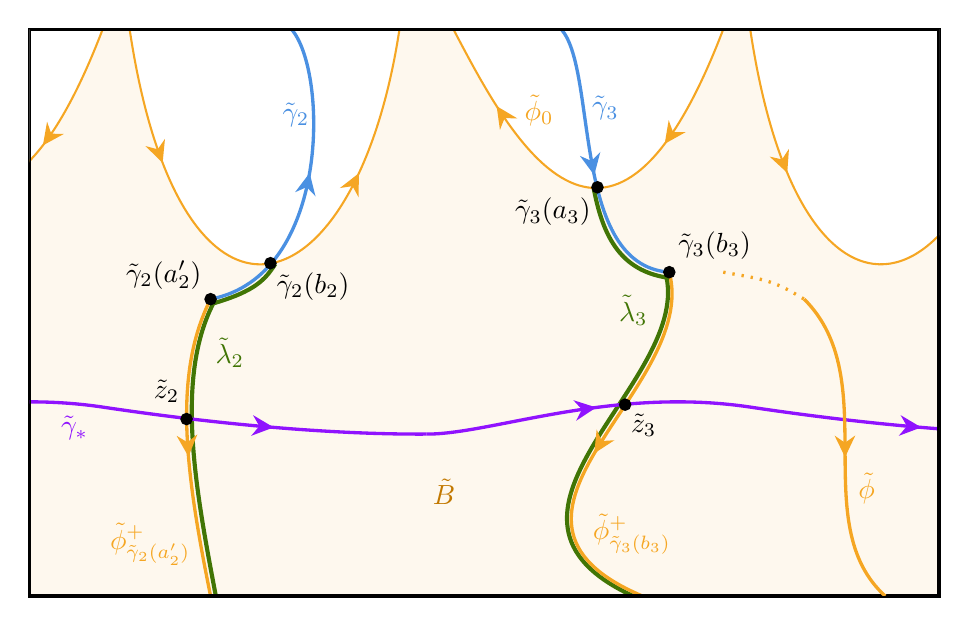
\begin{tikzpicture}[x=0.75pt,y=0.75pt,yscale=-1.3,xscale=1.3]

\draw [color={rgb, 255:red, 0; green, 0; blue, 0 },draw opacity=1][fill={rgb, 255:red, 245; green, 166; blue, 35 },fill opacity=0.08] (262.83,50) -- (600,50) -- (600,260) -- (262.83,260) -- cycle ;
\clip (262.83,50) rectangle (600,260);

\draw [color={rgb, 255:red, 245; green, 166; blue, 35 },draw opacity=1][fill={rgb, 255:red, 255; green, 255; blue, 255 },fill opacity=1][line width=0.75] (530,50).. controls (538.61,107.47) and (556.88,134.58).. (575.72,136.92).. controls (598.07,139.71) and (621.23,107.62).. (630,50) ;
\draw [shift={(543.72,103.2)}, rotate = 248.4] [fill={rgb, 255:red, 245; green, 166; blue, 35 },fill opacity=1][line width=0.08] [draw opacity=0] (8.04,-3.86) -- (0,0) -- (8.04,3.86) -- (5.34,0) -- cycle ;
\draw [shift={(616.41,100.13)}, rotate = 114.7] [fill={rgb, 255:red, 245; green, 166; blue, 35 },fill opacity=1][line width=0.08] [draw opacity=0] (8.04,-3.86) -- (0,0) -- (8.04,3.86) -- (5.34,0) -- cycle ;
\draw [color={rgb, 255:red, 245; green, 166; blue, 35 },draw opacity=1][fill={rgb, 255:red, 255; green, 255; blue, 255 },fill opacity=1][line width=0.75] (420,50).. controls (430.39,69.71) and (446.18,100.5).. (465.19,107.41).. controls (481.54,113.36) and (500.27,101.64).. (520,50) ;
\draw [shift={(436.01,78.45)}, rotate = 56.42] [fill={rgb, 255:red, 245; green, 166; blue, 35 },fill opacity=1][line width=0.08] [draw opacity=0] (8.04,-3.86) -- (0,0) -- (8.04,3.86) -- (5.34,0) -- cycle ;
\draw [shift={(498.3,92.43)}, rotate = 305.21] [fill={rgb, 255:red, 245; green, 166; blue, 35 },fill opacity=1][line width=0.08] [draw opacity=0] (8.04,-3.86) -- (0,0) -- (8.04,3.86) -- (5.34,0) -- cycle ;
\draw [color={rgb, 255:red, 245; green, 166; blue, 35 },draw opacity=1][fill={rgb, 255:red, 255; green, 255; blue, 255 },fill opacity=1][line width=0.75] (300,50).. controls (307.45,99.73) and (322.14,126.73).. (338.16,134.62).. controls (362.63,146.66) and (390.23,114.15).. (400,50) ;
\draw [shift={(312.22,99.48)}, rotate = 249.95] [fill={rgb, 255:red, 245; green, 166; blue, 35 },fill opacity=1][line width=0.08] [draw opacity=0] (8.04,-3.86) -- (0,0) -- (8.04,3.86) -- (5.34,0) -- cycle ;
\draw [shift={(384.97,103.33)}, rotate = 116.45] [fill={rgb, 255:red, 245; green, 166; blue, 35 },fill opacity=1][line width=0.08] [draw opacity=0] (8.04,-3.86) -- (0,0) -- (8.04,3.86) -- (5.34,0) -- cycle ;
\draw [color={rgb, 255:red, 65; green, 117; blue, 5 },draw opacity=1][line width=1.5] (354,136.96).. controls (350.35,142.46) and (347.03,146.89).. (331,151.57).. controls (316.72,179.62) and (324.52,220.93).. (332,260.28) ;
\draw [color={rgb, 255:red, 74; green, 144; blue, 226 },draw opacity=1] (360,50).. controls (373.48,65.44) and (374.68,141.44).. (330,150) ;
\draw [shift={(366.7,103.24)}, rotate = 101.43] [fill={rgb, 255:red, 74; green, 144; blue, 226 },fill opacity=1][line width=0.08] [draw opacity=0] (8.04,-3.86) -- (0,0) -- (8.04,3.86) -- (5.34,0) -- cycle ;
\draw [color={rgb, 255:red, 65; green, 117; blue, 5 },draw opacity=1][line width=1.5] (472,108.96).. controls (475.62,128.19) and (482.77,139.32).. (499,142).. controls (507,182.03) and (421,230.5).. (487.47,260.42) ;
\draw [color={rgb, 255:red, 74; green, 144; blue, 226 },draw opacity=1] (460,50).. controls (473.48,65.44) and (463.48,137.44).. (500,140) ;
\draw [shift={(472.19,104.05)}, rotate = 259.03] [fill={rgb, 255:red, 74; green, 144; blue, 226 },fill opacity=1][line width=0.08] [draw opacity=0] (8.04,-3.86) -- (0,0) -- (8.04,3.86) -- (5.34,0) -- cycle ;
\draw [color={rgb, 255:red, 245; green, 166; blue, 35 },draw opacity=1] (500,140).. controls (511.48,183.44) and (420.68,230.63).. (490,260) ;
\draw [shift={(472.2,207.15)}, rotate = 301.29] [fill={rgb, 255:red, 245; green, 166; blue, 35 },fill opacity=1][line width=0.08] [draw opacity=0] (8.04,-3.86) -- (0,0) -- (8.04,3.86) -- (5.34,0) -- cycle ;
\draw [color={rgb, 255:red, 245; green, 166; blue, 35 },draw opacity=1] (330,150).. controls (315.88,177.83) and (320.68,214.23).. (330,260) ;
\draw [shift={(321.81,208.38)}, rotate = 266.05] [fill={rgb, 255:red, 245; green, 166; blue, 35 },fill opacity=1][line width=0.08] [draw opacity=0] (8.04,-3.86) -- (0,0) -- (8.04,3.86) -- (5.34,0) -- cycle ;
\draw [color={rgb, 255:red, 144; green, 19; blue, 254 },draw opacity=1] (410,200).. controls (433.83,200.17) and (478.22,182.26).. (530,190).. controls (581.78,197.74) and (621.83,200.17).. (650,200) ;
\draw [shift={(472.91,190.14)}, rotate = 172.05] [fill={rgb, 255:red, 144; green, 19; blue, 254 },fill opacity=1][line width=0.08] [draw opacity=0] (8.04,-3.86) -- (0,0) -- (8.04,3.86) -- (5.34,0) -- cycle ;
\draw [shift={(593.38,197.52)}, rotate = 185.04] [fill={rgb, 255:red, 144; green, 19; blue, 254 },fill opacity=1][line width=0.08] [draw opacity=0] (8.04,-3.86) -- (0,0) -- (8.04,3.86) -- (5.34,0) -- cycle ;
\draw [color={rgb, 255:red, 144; green, 19; blue, 254 },draw opacity=1] (170,200).. controls (193.83,200.17) and (238.22,182.26).. (290,190).. controls (341.78,197.74) and (381.83,200.17).. (410,200) ;
\draw [shift={(232.91,190.14)}, rotate = 172.05] [fill={rgb, 255:red, 144; green, 19; blue, 254 },fill opacity=1][line width=0.08] [draw opacity=0] (8.04,-3.86) -- (0,0) -- (8.04,3.86) -- (5.34,0) -- cycle ;
\draw [shift={(353.38,197.52)}, rotate = 185.04] [fill={rgb, 255:red, 144; green, 19; blue, 254 },fill opacity=1][line width=0.08] [draw opacity=0] (8.04,-3.86) -- (0,0) -- (8.04,3.86) -- (5.34,0) -- cycle ;
\draw [fill={rgb, 255:red, 0; green, 0; blue, 0 },fill opacity=1] (471.7,108.54).. controls (471.7,107.61) and (472.45,106.86).. (473.38,106.86).. controls (474.31,106.86) and (475.06,107.61).. (475.06,108.54).. controls (475.06,109.47) and (474.31,110.22).. (473.38,110.22).. controls (472.45,110.22) and (471.7,109.47).. (471.7,108.54) -- cycle ;
\draw [fill={rgb, 255:red, 0; green, 0; blue, 0 },fill opacity=1] (350.51,136.67).. controls (350.51,135.74) and (351.26,134.99).. (352.19,134.99).. controls (353.12,134.99) and (353.87,135.74).. (353.87,136.67).. controls (353.87,137.6) and (353.12,138.35).. (352.19,138.35).. controls (351.26,138.35) and (350.51,137.6).. (350.51,136.67) -- cycle ;
\draw [fill={rgb, 255:red, 0; green, 0; blue, 0 },fill opacity=1] (319.42,194.44).. controls (319.42,193.51) and (320.17,192.75).. (321.1,192.75).. controls (322.02,192.75) and (322.78,193.51).. (322.78,194.44).. controls (322.78,195.36) and (322.02,196.12).. (321.1,196.12).. controls (320.17,196.12) and (319.42,195.36).. (319.42,194.44) -- cycle ;
\draw [fill={rgb, 255:red, 0; green, 0; blue, 0 },fill opacity=1] (481.96,189.09).. controls (481.96,188.17) and (482.71,187.41).. (483.64,187.41).. controls (484.57,187.41) and (485.32,188.17).. (485.32,189.09).. controls (485.32,190.02) and (484.57,190.78).. (483.64,190.78).. controls (482.71,190.78) and (481.96,190.02).. (481.96,189.09) -- cycle ;
\draw [fill={rgb, 255:red, 0; green, 0; blue, 0 },fill opacity=1] (498.32,140).. controls (498.32,139.07) and (499.07,138.32).. (500,138.32).. controls (500.93,138.32) and (501.68,139.07).. (501.68,140).. controls (501.68,140.93) and (500.93,141.68).. (500,141.68).. controls (499.07,141.68) and (498.32,140.93).. (498.32,140) -- cycle ;
\draw [fill={rgb, 255:red, 0; green, 0; blue, 0 },fill opacity=1] (328.32,150).. controls (328.32,149.07) and (329.07,148.32).. (330,148.32).. controls (330.93,148.32) and (331.68,149.07).. (331.68,150).. controls (331.68,150.93) and (330.93,151.68).. (330,151.68).. controls (329.07,151.68) and (328.32,150.93).. (328.32,150) -- cycle ;
\draw [color={rgb, 255:red, 245; green, 166; blue, 35 },draw opacity=1][fill={rgb, 255:red, 255; green, 255; blue, 255 },fill opacity=1][line width=0.75] (190,50).. controls (200.2,69.35) and (215.6,99.37).. (234.14,107.01).. controls (250.74,113.84) and (269.85,102.74).. (290,50) ;
\draw [shift={(205.67,77.91)}, rotate = 56.65] [fill={rgb, 255:red, 245; green, 166; blue, 35 },fill opacity=1][line width=0.08] [draw opacity=0] (8.04,-3.86) -- (0,0) -- (8.04,3.86) -- (5.34,0) -- cycle ;
\draw [shift={(267.85,93.02)}, rotate = 305.66] [fill={rgb, 255:red, 245; green, 166; blue, 35 },fill opacity=1][line width=0.08] [draw opacity=0] (8.04,-3.86) -- (0,0) -- (8.04,3.86) -- (5.34,0) -- cycle ;
\draw [color={rgb, 255:red, 0; green, 0; blue, 0 },draw opacity=1] (262.83,50) -- (600,50) -- (600,260) -- (262.83,260) -- cycle ;
\draw [color={rgb, 255:red, 245; green, 166; blue, 35 },draw opacity=1] (550,150).. controls (579.79,179.69) and (550.59,233.28).. (580,260) ;
\draw [shift={(565.15,208.56)}, rotate = 269.68] [fill={rgb, 255:red, 245; green, 166; blue, 35 },fill opacity=1][line width=0.08] [draw opacity=0] (8.04,-3.86) -- (0,0) -- (8.04,3.86) -- (5.34,0) -- cycle ;
\draw [color={rgb, 255:red, 245; green, 166; blue, 35 },draw opacity=1] [dash pattern={on 0.84pt off 2.51pt}] (520,140).. controls (536.19,142.89) and (538.19,142.89).. (550,150) ;

\draw (279.6,192.1) node [anchor=north] [inner sep=0.75pt] [color={rgb, 255:red, 144; green, 19; blue, 254 },opacity=1] {$\tilde{\gamma }_{*}$};
\draw (330.48,169.77) node [anchor=west] [inner sep=0.75pt] [font=\normalsize,color={rgb, 255:red, 65; green, 117; blue, 5 },opacity=1] {$\tilde{\lambda }_{2}$};
\draw (480,154.1) node [anchor=west] [inner sep=0.75pt] [font=\normalsize,color={rgb, 255:red, 65; green, 117; blue, 5 },opacity=1] {$\tilde{\lambda }_{3}$};
\draw (367.97,81.86) node [anchor=east] [inner sep=0.75pt] [font=\normalsize,color={rgb, 255:red, 74; green, 144; blue, 226 },opacity=1] {$\tilde{\gamma }_{2}$};
\draw (469.99,85.11) node [anchor=south west] [inner sep=0.75pt] [font=\normalsize,color={rgb, 255:red, 74; green, 144; blue, 226 },opacity=1] {$\tilde{\gamma }_{3}$};
\draw (472.21,111.16) node [anchor=north east] [inner sep=0.75pt] [font=\normalsize] {$\tilde{\gamma }_{3}(a_{3})$};
\draw (445,80) node [anchor=west] [inner sep=0.75pt] [font=\normalsize,color={rgb, 255:red, 245; green, 166; blue, 35 },opacity=1] {$\tilde \phi_0$};
\draw (353.19,138.65) node [anchor=north west][inner sep=0.75pt] [font=\normalsize] {$\tilde{\gamma }_{2}(b_{2})$};
\draw (319.75,189.59) node [anchor=south east] [inner sep=0.75pt] [font=\normalsize] {$\tilde{z}_{2}$};
\draw (484.44,191.17) node [anchor=north west][inner sep=0.75pt] [font=\normalsize] {$\tilde{z}_{3}$};
\draw (470.31,237.09) node [anchor=west] [inner sep=0.75pt] [font=\normalsize,color={rgb, 255:red, 245; green, 166; blue, 35 },opacity=1] {$\tilde \phi _{\tilde{\gamma }_{3}(b_{3})}^{+}$};
\draw (323.91,240.89) node [anchor=east] [inner sep=0.75pt] [font=\normalsize,color={rgb, 255:red, 245; green, 166; blue, 35 },opacity=1] {$\tilde \phi _{\tilde{\gamma }_{2}(a'_{2})}^{+}$};
\draw (411,215.4) node [anchor=north west][inner sep=0.75pt] [color={rgb, 255:red, 194; green, 120; blue, 0 },opacity=1] {$\tilde{B}$};
\draw (502,136.6) node [anchor=south west] [inner sep=0.75pt] [font=\normalsize] {$\tilde{\gamma }_{3}(b_{3})$};
\draw (328,147.6) node [anchor=south east] [inner sep=0.75pt] [font=\normalsize] {$\tilde{\gamma }_{2}(a'_{2})$};
\draw (568.67,220.17) node [anchor=west] [inner sep=0.75pt] [color={rgb, 255:red, 245; green, 166; blue, 35 },opacity=1] {$\tilde{\phi }$};
\end{tikzpicture}
\caption{The configuration of the proof of Lemma~\ref{lem:NotLeft}.\label{Fig:NotLeft}
}
\end{center}
\end{figure}


The sub-path of $\tilde\gamma_*$ that joins $\tilde z_2$ to $T^n\tilde z_3$ is disjoint from $\tilde\lambda_2$ and $T^n\tilde\lambda_3$ but at its endpoints, entering in $L_{\tilde B}(\tilde\lambda_2)$ at $\tilde z_2$ and leaving $R_{\tilde B}(T^n\tilde\lambda_3)$ at $T^n\tilde z_3$. Consequently the inclusion $\overline{L_{\tilde B}(T^n\tilde\lambda_3)}\subset L_{\tilde B}(\tilde\lambda_2)$ holds. Every leaf $\tilde\phi\subset L_{\tilde B}(\tilde\phi_{T^n\tilde z_3})$ is disjoint from $T^n\tilde\lambda_3$. It is contained in $L(T^n\tilde\lambda_3)$ because the sub-path of $\tilde\gamma_*$ that joins $\tilde\phi_{T^n(\tilde z_3)}$ to $\tilde\phi$ is disjoint from $T^n\tilde\lambda_3$ but at $T^n\tilde z_3$ and enters in $L_{\tilde B}(T^n\tilde\lambda_3)$ at $T^n\tilde z_3$. The contradiction comes from the fact that $\tilde \phi$ must intersect $\tilde\gamma_2\vert_{[a'_2,b_2)}$ because $\tilde\phi\subset L_{\tilde B}(\tilde\phi_{\tilde z_2}).$
\end{proof}

\begin{lemm}\label{Lem:ProjAnnulus}
The set $B$ is an open annulus of $\Sigma$.
\end{lemm}

\begin{proof}
Suppose it is not. Then there exists a deck transformation $T'\notin\langle T\rangle$ of $\tilde\Sigma$ such that $T'\tilde B\cap \tilde B\neq \emptyset$. As $\tilde B$ is the set of leaves met by $\tilde\gamma_*$, it implies the existence of $t\in\R$ such that $T'\tilde\gamma_*(t) \in \tilde B$. The line $\tilde\gamma_*$ lifts the simple loop $\Gamma_*$ and so we have $T'\tilde\gamma_*\cap \tilde\gamma_*=\emptyset$. Moreover, there is at least one leaf of $\tilde{\F}$ that is met both by $\tilde\gamma_*$ and $T'\tilde\gamma_*$. Consequently, one of the following inclusions $\overline{L(T'\tilde\gamma_*)}\subset L(\tilde\gamma_*)$, $\overline{L(\tilde\gamma_*)}\subset L(T'\tilde\gamma_*)$ holds. Replacing $T'$ by $T'{}^{-1}$ if necessary, one can suppose that the first inclusion holds, which implies that $T'\tilde\gamma_*\subset L(\tilde\gamma_*)$.

Note that $T'\tilde\gamma_*$ cannot accumulate on $\tilde\gamma_*$ (neither positively nor negatively) because the natural lift $\gamma_*$ of $\Gamma_*$ is recurrent and so, by Lemma~\ref{LemEquivSubpath}, cannot accumulate on itself. Moreover it cannot be equivalent to $\tilde\gamma_*$ neither at $+\infty$ nor at $-\infty$ (by using Lemma~\ref{LemEquivSubpath}). It cannot cross $\tilde B$ because $T'\tilde\gamma_*\cap \tilde\gamma_*=\emptyset$. It remains to prove that it cannot visit $\tilde B$.

Using the fact that $T'\tilde\gamma_*\subset L(\tilde\gamma_*)$, the line $T'\tilde\gamma_*$ must visit~~$\tilde B$ by the left if it visits~$\tilde B$. This contradicts Lemma~\ref{lem:NotLeft}: no transverse trajectory enters in $\tilde B$ by the left side.
\end{proof}

To prove Proposition~\ref{prop: nontransitivity3}, it remains to prove that $\gamma_1$ is entirely contained in $B$ (which will imply that $\tilde\gamma_1$ is entirely contained in $\tilde B$). But this is implied by the facts that $\gamma_1\vert_{[a_1,+\infty)}$ is contained in $B$ and that $\gamma_1$ is recurrent. This finishes the proof of Proposition~\ref{prop: nontransitivity3}.
\end{proof}

